\documentclass[10pt]{article}
\usepackage[utf8]{inputenc}
\usepackage[T1]{fontenc}
\usepackage{hyperref}
\hypersetup{colorlinks=true, linkcolor=blue, filecolor=magenta, urlcolor=cyan,}
\urlstyle{same}
\usepackage{amsmath}
\usepackage{amsfonts}
\usepackage{amssymb}
\usepackage[version=4]{mhchem}
\usepackage{stmaryrd}
\usepackage{bbold}
\usepackage{mathtools}
\usepackage{graphicx}
\usepackage[export]{adjustbox}
\graphicspath{ {./images/} }

\title{Online Appendix: \\
 The Four Equation New Keynesian Model * \\
 \textbackslash author\{ Eric Sims }

\author{Ji Zhang\\
Tsinghua PBCSF}
\date{}


%New command to display footnote whose markers will always be hidden
\let\svthefootnote\thefootnote
\newcommand\blfootnotetext[1]{%
  \let\thefootnote\relax\footnote{#1}%
  \addtocounter{footnote}{-1}%
  \let\thefootnote\svthefootnote%
}

%Overriding the \footnotetext command to hide the marker if its value is `0`
\let\svfootnotetext\footnotetext
\renewcommand\footnotetext[2][?]{%
  \if\relax#1\relax%
    \ifnum\value{footnote}=0\blfootnotetext{#2}\else\svfootnotetext{#2}\fi%
  \else%
    \if?#1\ifnum\value{footnote}=0\blfootnotetext{#2}\else\svfootnotetext{#2}\fi%
    \else\svfootnotetext[#1]{#2}\fi%
  \fi
}

\begin{document}
\maketitle
 \\
 Jing Cynthia Wu \\
 Notre Dame and NBER Notre Dame and NBER\}

The online appendix contains the following sections to supplement Sims et al. (forthcoming):\\
A: The Full Non-Linear Model: Here we show the full set of non-linear equilibrium conditions underlying our linearized four equation model.

B: Details of the Linearized Model: Here we show the full set of linearized equilibrium conditions of the model, and discuss how to reduce these down to the four equations presented in the text.

C: Determinacy of Interest Rate Rules: Here we derive conditions on the parameters of policy rules necessary for a unique rational expectations equilibrium.

D: Potential, Flexible Price, and Efficient Output: Here we derive expressions for potential, flexible price, and efficient output in our four equation model.

E: Model Calibration: Here we provide more detail on the baseline calibration of our four equation model.

F: Robustness: Here we compute impulse responses to shocks under a couple of different specifications of our four equation model.

G: Optimal Monetary Policy: Here we derive optimal equilibrium conditions for a central bank operating under discretion and provide formal proofs for some of the theorems and lemmas in the paper.

H: Additional Results: Here we show a few additional quantitative results related to optimal policy.

\footnotetext{*This material is based upon work supported by the National Science Foundation under Grant No. SES1949107. Correspondence: \href{mailto:esims1@nd.edu}{esims1@nd.edu}, \href{mailto:cynthia.wu@nd.edu}{cynthia.wu@nd.edu}, \href{mailto:zhangji@pbcsf.tsinghua.edu.cn}{zhangji@pbcsf.tsinghua.edu.cn}.
}\section*{A The Full Non-Linear Model}
This appendix describes the full set of non-linear equilibrium conditions of the model.\\
The optimality condition for retail firms may be re-written in stationary terms by defining $p_{*, t}=P_{*, t} / P_{t}, x_{1, t}=X_{1, t} / P_{t}^{\epsilon}$, and $x_{2, t}=X_{2, t} / P_{t}^{\epsilon-1}:$\\
\begin{gather*}
p_{*, t}=\frac{\epsilon}{\epsilon-1} \frac{x_{1, t}}{x_{2, t}}  \tag{A.1}\\
x_{1, t}=p_{m, t} Y_{t}+\phi \mathbb{E}_{t} \Lambda_{t, t+1} \Pi_{t+1}^{\epsilon} x_{1, t+1}  \tag{A.2}\\
x_{2, t}=Y_{t}+\phi \mathbb{E}_{t} \Lambda_{t, t+1} \Pi_{t}^{\epsilon-1} x_{2, t+1} \tag{A.3}
\end{gather*}

The aggregate inflation rate evolves according to:

\begin{equation*}
1=(1-\phi) p_{*, t}^{1-\epsilon}+\phi \Pi_{t}^{\epsilon-1} \tag{A.4}
\end{equation*}

Price dispersion evolves according to:

\begin{equation*}
v_{t}^{p}=(1-\phi) p_{*, t}^{-\epsilon}+\phi \Pi_{t}^{\epsilon} v_{t-1}^{p} \tag{A.5}
\end{equation*}

Define lowercase variables as real values of nominal bonds, i.e. $b_{t}=B_{t} / P_{t}$. The balance sheet condition of the FI may be written:

\begin{equation*}
Q_{t} b_{t}^{F I}+r e_{t}=s_{t}+X_{t}^{F I} \tag{A.6}
\end{equation*}

The leverage constraint of the FI may be written:

\begin{equation*}
Q_{t} b_{t}^{F I} \leq \Theta_{t} \bar{X}^{F I} \tag{A.7}
\end{equation*}

The central bank's balance sheet can be written:

\begin{equation*}
Q_{t} t_{t}^{c b}=r e_{t} \tag{A.8}
\end{equation*}

Similarly, the market-clearing condition for long term bonds in real terms is:

\begin{equation*}
b_{t}=b_{t}^{F I}+b_{t}^{c b} \tag{A.9}
\end{equation*}

The auxiliary $Q E_{t}$ variable is just the real value of the central bank's long bond portfolio:

\begin{equation*}
Q E_{t}=Q_{t} t_{t}^{c b} \tag{A.10}
\end{equation*}

Under our assumption on the transfer from parent to child, the consumption of the child may be written:

\begin{equation*}
C_{b, t}=Q_{t} b_{t} \tag{A.11}
\end{equation*}

$A_{t}$ and $\Theta_{t}$ obey stationary $\operatorname{AR}(1)$ processes, where the non-stochastic steady state value of productivity is normalized to unity and $\Theta$ denotes the non-stochastic steady state value of leverage.\\
\begin{gather*}
\ln A_{t}=\rho_{A} \ln A_{t-1}+s_{A} \varepsilon_{A, t}  \tag{A.12}\\
\ln \Theta_{t}=\left(1-\rho_{\theta}\right) \ln \Theta+\rho_{\theta} \ln \Theta_{t-1}+s_{\theta} \varepsilon_{\theta, t} \tag{A.13}
\end{gather*}

To close the model, it is necessary to specify rules for the policy rate and the central bank's\\
bond holdings. For the analysis in Subsection 2.3, we assume that the policy rate is set according to a Taylor rule and that the central bank's bond holdings obey an exogenous AR(1) process:\\
\begin{gather*}
\ln R_{t}^{s}=\left(1-\rho_{r}\right) \ln R^{s}+\left(1-\rho_{r}\right)\left[\phi_{\pi}\left(\ln \Pi_{t}-\ln \Pi\right)+\phi_{x}\left(\ln Y_{t}-\ln Y_{t}^{*}\right)\right]+s_{r} \varepsilon_{r, t}  \tag{A.14}\\
\ln Q E_{t}=\left(1-\rho_{q}\right) \ln Q E+\rho_{q} \ln Q E_{t-1}+s_{q} \varepsilon_{q, t} \tag{A.15}
\end{gather*}

In (A.14)-(A.15), $R^{s}$ and $Q E$ denote the non-stochastic steady state values of the policy rate and the central bank's balance sheet, respectively.\\
$Y_{t}^{*}$ can be found by solving the full system of equations assuming price flexibility $(\phi=0)$ where the credit shock is constant, i.e. $\Theta_{t}=\Theta$. Taking $Y_{t}^{*}$ as given, the output gap is then:

\begin{equation*}
\ln X_{t}=\ln Y_{t}-\ln Y_{t}^{*} \tag{A.16}
\end{equation*}

The optimality conditions for the parent household, (2.5)-(2.7); the definition of the return on the long bond, (2.12); the optimality conditions for the child, (2.13)-(2.14); the optimality conditions for the FI, (2.19)-(2.20); the balance sheet condition for the FI and the leverage constraint re-written in real terms, (A.6)-(A.7); the labor demand condition for the wholesale firm, (2.27); the optimality condition for optimal price-setting for retailers, re-written in stationary form, (A.1)-(A.3); the market-clearing condition and aggregate production function, (2.30)-(2.31); the central bank's policy rule for $R_{t}^{r e}$, (A.14); the central bank's balance sheet and definition of the $Q E_{t}$ variable, (A.8) and (A.10); the central bank's QE rule, (A.15); the consumption of the child, (A.11); the bond market-clearing condition, (A.9); the evolution of inflation and price dispersion, (A.4)-(A.5); the definition of the output gap, (A.16); and the exogenous processes (A.12)-(A.3) constitute twentyseven variables, $\left\{L_{t}, C_{t}, w_{t}, \Lambda_{t-1, t}, R_{t}^{s}, \Pi_{t}, \Lambda_{b, t-1, t}, R_{t}^{b}, Q_{t}, b_{t}^{F I}, \Theta_{t}, r e_{t}, s_{t}, \Omega_{t}, R_{t}^{r e}, p_{*, t}, x_{1, t}, x_{2, t}, p_{m, t}, Y_{t}, A_{t}, C_{b, t}\right.$, $\left.v_{t}^{p}, b_{c b, t}, b_{t}, Q E_{t}, X_{t}\right\}$ in twenty-seven equations.

\section*{B Details of the Linearized Model}
This Appendix provides details of the linearization of the non-linear model, the equilibrium conditions for which are given in Appendix A. Where possible, lowercase variables denote log deviations from steady state, e.g. $\theta_{t}=\ln \Theta_{t}-\ln \Theta$. Where the corresponding level variable is already lowercase, a "hat" is put atop the relevant variable to denote a log deviation from steady state, e.g. $\widehat{p}_{m, t}=\ln p_{m, t}-\ln p_{m}$. Variables without a time subscript denote non-stochastic steady state values. The model is linearized about a steady state with zero trend inflation (i.e. $\Pi=1$ ) where the leverage constraint on intermediaries binds. The complete list of linearized equilibrium conditions are as follows:\\
\begin{gather*}
\chi l_{t}=-\sigma c_{t}+\widehat{w}_{t}  \tag{B.1}\\
\lambda_{t-1, t}=-\sigma\left(c_{t}-c_{t-1}\right)  \tag{B.2}\\
0=\mathbb{E}_{t} \lambda_{t, t+1}+r_{t}^{s}-\mathbb{E}_{t} \pi_{t+1}  \tag{B.3}\\
\lambda_{b, t-1, t}=-\sigma\left(c_{b, t}-c_{b, t-1}\right)  \tag{B.4}\\
r_{t}^{b}=\frac{\kappa}{R^{b}} q_{t}-q_{t-1}  \tag{B.5}\\
0=\mathbb{E}_{t} \lambda_{b, t, t+1}+\mathbb{E}_{t} r_{t+1}^{b}-\mathbb{E}_{t} \pi_{t+1} \tag{B.6}
\end{gather*}\\
\begin{align*}
& q_{t}+\widehat{b}_{t}^{F I}=\theta_{t}  \tag{B.7}\\
& {\left[Q b^{F I}(1-\kappa)\right] q_{t}+Q b^{F I} \widehat{b}_{t}^{F I}-\kappa Q b^{F I} \widehat{b}_{t-1}^{F I}+\kappa Q b^{F I} \pi_{t}+r e \cdot \widehat{r e}{ }_{t}=s \cdot \widehat{s}_{t}}  \tag{B.8}\\
& \mathbb{E}_{t} \lambda_{t, t+1}-\mathbb{E}_{t} \pi_{t+1}+\frac{R^{b}}{s p} \mathbb{E}_{t} r_{t+1}^{b}-\frac{R^{s}}{s p} r_{t}^{s}=\omega_{t}  \tag{B.9}\\
& r_{t}^{r e}=r_{t}^{s}  \tag{B.10}\\
& \widehat{p}_{*, t}=\widehat{x}_{1, t}-\widehat{x}_{2, t}  \tag{B.11}\\
& \widehat{x}_{1, t}=(1-\phi \beta) \widehat{p}_{m, t}+(1-\phi \beta) y_{t}+\phi \beta \mathbb{E}_{t} \lambda_{t, t+1}+\epsilon \phi \beta \mathbb{E}_{t} \pi_{t+1}+\phi \beta \mathbb{E}_{t} \widehat{x}_{1, t+1}  \tag{B.12}\\
& \widehat{x}_{2, t}=(1-\phi \beta) y_{t}+\phi \beta \mathbb{E}_{t} \lambda_{t, t+1}+(\epsilon-1) \phi \beta \mathbb{E}_{t} \pi_{t+1}+\phi \beta \mathbb{E}_{t} \widehat{x}_{2, t+1}  \tag{B.13}\\
& \widehat{w}_{t}=\widehat{p}_{m, t}+a_{t}  \tag{B.14}\\
& (1-z) c_{t}+z c_{b, t}=y_{t}  \tag{B.15}\\
& \widehat{v}_{t}^{p}+y_{t}=a_{t}+l_{t}  \tag{B.16}\\
& \widehat{v}_{t}^{p}=0  \tag{B.17}\\
& \pi_{t}=\frac{1-\phi}{\phi} \widehat{p}_{*, t}  \tag{B.18}\\
& q_{t}+\widehat{b}_{t}^{c b}=\widehat{r e}_{t}  \tag{B.19}\\
& \widehat{b}_{t}=\frac{b^{F I}}{b} \widehat{b}_{t}^{F I}+\frac{b^{c b}}{b} \widehat{b}_{t}^{c b}  \tag{B.20}\\
& c_{b, t}=q_{t}+\widehat{b}_{t}  \tag{B.21}\\
& q e_{t}=\rho_{q} q e_{t-1}+s_{q} \varepsilon_{q, t}  \tag{B.22}\\
& a_{t}=\rho_{A} a_{t-1}+s_{A} \varepsilon_{A, t}  \tag{B.23}\\
& \theta_{t}=\rho_{\theta} \theta_{t-1}+s_{\theta} \varepsilon_{\theta, t}  \tag{B.24}\\
& r_{t}^{r e}=\rho_{r} r_{t-1}^{r e}+\left(1-\rho_{r}\right)\left[\phi_{\pi} \pi_{t}+\phi_{x} x_{t}\right]+s_{r} \varepsilon_{r, t}  \tag{B.25}\\
& q e_{t}=\widehat{r e}_{t}  \tag{B.26}\\
& x_{t}=y_{t}-y_{t}^{*} \tag{B.27}
\end{align*}

This is twenty-seven equations in $\left\{l_{t}, c_{t}, \widehat{w}_{t}, \lambda_{t-1, t}, r_{t}^{s}, \pi_{t}, \lambda_{b, t-1, t}, r_{t}^{b}, q_{t}, \widehat{b}_{t}^{F I}, \theta_{t}, \widehat{r e}_{t}, \widehat{s}_{t}, \omega_{t}, r_{t}^{r e}\right.$, $\left.\widehat{p}_{*, t}, \widehat{x}_{1, t}, \widehat{x}_{2, t}, \widehat{p}_{m, t}, y_{t}, a_{t}, c_{b, t}, \widehat{v}_{t}^{p}, \widehat{b}_{t}^{c b}, \widehat{b}_{t}, q e_{t}, x_{t}\right\}$ in twenty-seven variables.

The model can be reduced to the equations presented in Subsection 2.1 as follows. First, (B.10) can be used to eliminate $r_{t}^{r e}$, so that the policy rule may be written as (2.34) in terms of $r_{t}^{s}$. Second, (B.11)-(B.13) can be combined with (B.18), which yields the textbook New Keynesian Phillips curve expressed as a function of marginal cost, where $\gamma=\frac{(1-\phi)(1-\phi \beta)}{\phi}$ :

\begin{equation*}
\pi_{t}=\gamma \widehat{p}_{m, t}+\beta \mathbb{E}_{t} \pi_{t+1} \tag{B.28}
\end{equation*}

Combining (B.1) with (B.14) and (B.16), making note of the fact that $\widehat{v}_{t}^{p}=0$ around a zero inflation steady state, yields:

\begin{equation*}
\widehat{p}_{m, t}=\chi y_{t}-(1+\chi) a_{t}+\sigma c_{t} \tag{B.29}
\end{equation*}

Making use of (B.15) allows us to write this as:

\begin{equation*}
\widehat{p}_{m, t}=\frac{\chi(1-z)+\sigma}{1-z} y_{t}-(1+\chi) a_{t}-\frac{\sigma z}{1-z} c_{b, t} \tag{B.30}
\end{equation*}

Combining (B.19)-(B.21) with (B.26) allows us to write:

\begin{equation*}
c_{b, t}=\frac{b^{F I}}{b}\left(q_{t}+\widehat{b}_{t}^{F I}\right)+\frac{b^{c b}}{b} q e_{t} \tag{B.31}
\end{equation*}

Defining $\bar{b}^{F I}=b^{F I} / b$ and $\bar{b}^{c b}=b^{c b} / b$ (i.e. the fraction of total bonds held by financial intermediaries and the central bank, respectively, in steady state), and making use of the binding leverage constraint, (B.7), leaves:

\begin{equation*}
c_{b, t}=\bar{b}^{F I} \theta_{t}+\bar{b}^{c b} q e_{t} \tag{B.32}
\end{equation*}

Plugging (B.32) into (B.30) then gives:

\begin{equation*}
\widehat{p}_{m, t}=\frac{\chi(1-z)+\sigma}{1-z} y_{t}-(1+\chi) a_{t}-\frac{\sigma z}{1-z}\left[\bar{b}^{F I} \theta_{t}+\bar{b}^{c b} q e_{t}\right] \tag{B.33}
\end{equation*}

Define the hypothetical natural rate of output, $y_{t}^{*}$, as the level of output consistent with flexible prices and no credit market shocks. That is, $y_{t}^{*}$ is the level of output consistent with $\widehat{p}_{m, t}=\theta_{t}=$ $q e_{t}=0$, or:

\begin{equation*}
y_{t}^{*}=\frac{(1+\chi)(1-z)}{\chi(1-z)+\sigma} a_{t} \tag{B.34}
\end{equation*}

But then, using (B.27), we can write marginal cost as:

\begin{equation*}
\widehat{p}_{m, t}=\frac{\chi(1-z)+\sigma}{1-z} x_{t}-\frac{\sigma z}{1-z}\left[\bar{b}^{F I} \theta_{t}+\bar{b}^{c b} q e_{t}\right] \tag{B.35}
\end{equation*}

Plugging (B.35) into (B.28), defining $\zeta=\frac{\chi(1-z)+\sigma}{1-z}$, yields (2.2).\\
To derive the IS equation, combine (B.2)-(B.4) with (B.6) and (B.15). Doing so yields:

\begin{equation*}
y_{t}=\mathbb{E}_{t} y_{t+1}-\frac{1-z}{\sigma}\left(r_{t}^{s}-\mathbb{E}_{t} \pi_{t+1}\right)-\frac{z}{\sigma}\left(\mathbb{E}_{t} r_{t+1}^{b}-\mathbb{E}_{t} \pi_{t+1}\right) \tag{B.36}
\end{equation*}

But from the Euler equation for the impatient household, along with the "full bailout" assumption embodied in (B.21), we can write:

\begin{equation*}
\mathbb{E}_{t} r_{t+1}^{b}-\mathbb{E}_{t} \pi_{t+1}=\sigma\left[\mathbb{E}_{t} c_{b, t+1}-c_{b, t}\right]=\sigma\left[\bar{b}^{F I}\left(\mathbb{E}_{t} \theta_{t+1}-\theta_{t}\right)+\bar{b}^{c b}\left(\mathbb{E}_{t} q e_{t+1}-q e_{t}\right)\right] \tag{B.37}
\end{equation*}

Combining (B.37) with (B.36) yields:

\begin{equation*}
y_{t}=\mathbb{E}_{t} y_{t+1}-\frac{1-z}{\sigma}\left(r_{t}^{s}-\mathbb{E}_{t} \pi_{t+1}\right)-z\left[\bar{b}^{F I}\left(\mathbb{E}_{t} \theta_{t+1}-\theta_{t}\right)+\bar{b}^{c b}\left(\mathbb{E}_{t} q e_{t+1}-q e_{t}\right)\right] \tag{B.38}
\end{equation*}

Note that an alternative, and arguably more intuitive, way to write the IS expression is based on a simple algebraic manipulation of (B.36):

\begin{equation*}
y_{t}=\mathbb{E}_{t} y_{t+1}-\frac{1}{\sigma}\left(r_{t}^{s}-\mathbb{E}_{t} \pi_{t+1}\right)-\frac{z}{\sigma}\left(\mathbb{E}_{t} r_{t+1}^{b}-r_{t}^{s}\right) \tag{B.39}
\end{equation*}

(B.39) is the familiar IS/Euler equation, written in terms of output rather than the output gap, appended with a term equal to the long-short interest rate spread, i.e. $\mathbb{E}_{t} r_{t+1}^{b}-r_{t}^{s}$.

The natural rate of interest, $r_{t}^{*}$, is defined as the real rate consistent with the IS equation holding at the natural rate of output absent credit shocks. This implies that:

\begin{equation*}
r_{t}^{*}=\frac{\sigma}{1-z}\left(\mathbb{E}_{t} y_{t+1}^{*}-y_{t}^{*}\right) \tag{B.40}
\end{equation*}

Adding and subtracting $y_{t}^{*}$ and $\mathbb{E}_{t} y_{t+1}^{*}$ from both sides of (B.38) and re-arranging yields (2.1). Making use of (B.23), allows one to write an $\operatorname{AR}(1)$ process for $r_{t}^{*}$ as in (2.36), where $\rho_{f}=\rho_{A}$ and $s_{f}=\frac{\sigma\left(\rho_{A}-1\right)(1+\chi)}{\chi(1-z)+\sigma}$.

\begin{equation*}
r_{t}^{*}=\frac{\sigma\left(\rho_{A}-1\right)}{1-z} y_{t}^{*} \tag{B.41}
\end{equation*}

Computing the dynamics of $x_{t}, \pi_{t}$, and $r_{t}^{s}$ does not require keeping track of $y_{t}, y_{t}^{*}, q_{t}, r_{t}^{b}, \omega_{t}, \widehat{s}_{t}$, $\widehat{b}_{t}^{F I}, \widehat{b}_{t}, \widehat{b}_{c b, t}$ or $c_{b, t}$. Given the solution for $x_{t}, \pi_{t}$, and $r_{t}^{s}$, the dynamics of these variables can be computed using the full system, (B.1)-(B.27).

\section*{C Determinacy of Interest Rate Rules}
The linearized four equation model as laid out in Section 2 - as captured by the IS equation, (2.1), the Phillips curve, (2.2), and rules for the policy rate, (2.34), and the central bank's long bond portfolio, (2.35) - has exactly the same requirements for equilibrium determinacy as the textbook three equation model when the central bank's long bond portfolio is exogenous.

For the purposes of examining equilibrium determinacy, one can treat purely exogenous variable as constant - e.g. set $r_{t}^{*}=\theta_{t}=0$, and set $q e_{t}=0$ since we are thinking of it as exogenous for now. Define a vector of variables, $\mathbf{z}_{t}=\left[\begin{array}{lll}\pi_{t} & x_{t} & r_{t-1}^{s}\end{array}\right]^{\prime}$. This vector of variables evolves according to:

\begin{equation*}
\mathbb{E}_{t} \mathbf{z}_{t+1}=\mathbf{A} \mathbf{z}_{t} \tag{C.1}
\end{equation*}

where:\\
\textbackslash mathbf\{A\}=\textbackslash left(\[
\begin{array}{ccc}
1+\frac{1-z}{\sigma}\left(\phi_{x}\left(1-\rho_{r}\right)+\frac{\gamma \zeta}{\beta}\right) & \frac{1-z}{\sigma}\left(\phi_{\pi}\left(1-\rho_{r}\right)-\beta^{-1}\right) & \frac{(1-z) \rho_{r}}{\sigma}  \tag{C.2}\\
-\frac{\gamma \zeta}{\beta} & \beta^{-1} & 0 \\
\phi_{x}\left(1-\rho_{r}\right) & \phi_{\pi}\left(1-\rho_{r}\right) & \rho_{r}
\end{array}
\]\textbackslash right) .

The proof of determinacy follows Woodford (2003), Appendix C. The vector $\mathbf{z}_{t}$ includes two forward-looking variables, $\pi_{t}$ and $x_{t}$, and one state variable, $r_{t-1}^{s}$. For a unique rational expectations equilibrium, there must be exactly two unstable eigenvalues of $\mathbf{A}$. The characteristic roots of $\mathbf{A}$ satisfy:

\begin{equation*}
\mathcal{P}(\mu)=\mu^{3}+A_{2} \mu^{2}+A_{1} \mu+A_{0}=0 \tag{C.3}
\end{equation*}

where:\\
\begin{align*}
A_{0} & =-\operatorname{det}(\mathbf{A})  \tag{C.4}\\
A_{1} & =\frac{1}{2}\left(\operatorname{tr}\left(\mathbf{A}^{2}\right)-\operatorname{tr}(\mathbf{A})^{2}\right)  \tag{C.5}\\
A_{2} & =-\operatorname{tr}(\mathbf{A}) \tag{C.6}
\end{align*}

For exactly two unstable eigenvalues, the following conditions must be satisfied:\\
\[
\begin{array}{r}
1+A_{2}+A_{1}+A_{0}>0 \\
-1+A_{2}-A_{1}+A_{0}<0 \\
A_{0}^{2}-A_{0} A_{2}+A_{1}-1>0 \tag{C.9}
\end{array}
\]\\
(C.8) is automatically satisfied given assumptions on signs of the parameters. A necessary and sufficient condition for (C.7) and (C.9) being satisfied is that:

\begin{equation*}
\phi_{\pi}\left(1-\rho_{r}\right)+\frac{1-\beta}{\gamma \zeta} \phi_{x}\left(1-\rho_{r}\right)>1-\rho_{r} \tag{C.10}
\end{equation*}

or, more compactly:

\begin{equation*}
\phi_{\pi}+\frac{1-\beta}{\gamma \zeta} \phi_{x}>1 \tag{C.11}
\end{equation*}

This is the same condition required for equilibrium determinacy in the three equation New Keynesian model, subject to the caveat that the slope coefficient in the Phillips curve, $\gamma \zeta$, is slightly different in the four equation model. (C.11) requires that the central bank react sufficiently aggressively to endogenous variables inflation and the output gap. Intuitively, so long as the central bank's long bond portfolio is exogenous, in terms of endogenous variables the four equation model takes exactly the same form as the three equation model, only with slightly different coefficients on the output gap in the Phillips curve and on the real interest rate in the IS equation. Hence, it should not be surprising that the condition on the parameters of the interest rate rule for determinacy is the same as in the three equation model.

When we consider an endogenous QE rule, as in Section 4, the system of variables expands to four: $\mathbf{z}_{t}=\left[\begin{array}{llll}\pi_{t} & x_{t} & r_{t-1}^{s} & q e_{t-1}\end{array}\right]^{\prime}$. The system of endogenous variables may be written:

\begin{equation*}
\mathbf{B}_{1} \mathbb{E}_{t} \mathbf{z}_{t+1}=\mathbf{B}_{2} \mathbf{z}_{t} \tag{C.12}
\end{equation*}

where:\\
\begin{gather*}
\mathbf{B}_{2}=\left(\begin{array}{cccc}
\beta & 0 & 0 & -\frac{z \gamma \sigma}{1-z} \bar{b}^{c b} \\
\frac{1-z}{\sigma}-z \bar{b}^{c b}\left(1-\rho_{q}\right) \lambda_{\pi} & 1-z \bar{b}^{c b}\left(1-\rho_{q}\right) \lambda_{x} & -\frac{1-z}{\sigma} & z \bar{b}^{c b}\left(1-\rho_{q}\right) \\
0 & 0 & 1 & 0 \\
0 & 0 & 0 & 1
\end{array}\right)  \tag{C.13}\\
\mathbf{B}_{1}=\left(\begin{array}{cccc}
1 & -\gamma \zeta & 0 & 0 \\
0 & 1 & 0 & 0 \\
\left(1-\rho_{r}\right) \phi_{\pi} & \left(1-\rho_{r}\right) \phi_{x} & \rho_{r} & 0 \\
\left(1-\rho_{q}\right) \lambda_{\pi} & \left(1-\rho_{q}\right) \lambda_{x} & 0 & \rho_{q}
\end{array}\right) \tag{C.14}
\end{gather*}

We then have:

\begin{equation*}
\mathbb{E}_{t} \mathbf{z}_{t+1}=\mathbf{A} \mathbf{z}_{t} \tag{C.15}
\end{equation*}

where:

\begin{equation*}
\mathbf{A}=\mathbf{B}_{1}^{-1} \mathbf{B}_{2} . \tag{C.16}
\end{equation*}

As discussed in Section 4, we numerically characterize restrictions on policy rule reaction coefficients for equilibrium determinacy (i.e. for there to be exactly two unstable eigenvalues in $\mathbf{A}$ ).

\section*{D Potential, Flexible Price, and Efficient Output}
As noted above, we define potential output, $y_{t}^{*}$, as the level of output consistent with flexible prices and no credit market shocks. It is given by (B.34). One could alternatively define flexible price output, $y_{t}^{f}$, as the level of output consistent with flexible prices only. This would satisfy:

\begin{equation*}
y_{t}^{f}=\frac{(1-z)(1+\chi)}{\chi(1-z)+\sigma} a_{t}+\frac{\sigma z}{\chi(1-z)+\sigma}\left[\bar{b}^{F I} \theta_{t}+\bar{b}^{c b} q e_{t}\right] \tag{D.1}
\end{equation*}

The difference between (D.1) and (B.34) is that credit market disturbances - both $\theta_{t}$ as well as $q e_{t}$ - impact flexible price output but not potential output. If we were to instead define the output gap as $x_{t}^{f}=y_{t}-y_{t}^{f}$, the Phillips curve representation would be:

\begin{equation*}
\pi_{t}=\gamma \zeta x_{t}^{f}+\beta \mathbb{E}_{t} \pi_{t+1} \tag{D.2}
\end{equation*}

In other words, written in terms of flexible price output, the Phillips curve, (D.2), features no endogenous cost-push wedge related to credit market disturbances. The cost-push wedge comes from defining potential output as not featuring credit market disturbances in addition to price flexibility. Credit market shocks drive a wedge between $y_{t}^{*}$ and $y_{t}^{f}$, in a similar way to how markup shocks are often used to justify a wedge between flexible price and efficient output - and a corresponding cost-push wedge in the Phillips curve - in the standard three equation model.

To be clear, (D.2) and (2.2) are equivalent ways to describe the supply-side of the model. If one prefers to work with (D.2), one simply needs to write the IS equation and exogenous processes in terms of $x_{t}^{f}, y_{t}^{f}$ and $r_{t}^{f}$ instead of $x_{t}, y_{t}^{*}$, and $r_{t}^{*}$. We prefer working with the specification in the text, using our definition of potential output, because it aligns closer to the notion of efficient output, which is ultimately what is relevant for welfare. Our model features two time-varying welfare-relevant distortions, not one as in the standard New Keynesian model.

We can motivate our notion of potential output, $y_{t}^{*}$, as coinciding with efficient output under a particular welfare criterion. Suppose that the planner's objective is to maximize the utility of the parent, (2.3), subject to perfectly smoothing the child's consumption at some constant level, $\bar{C}_{b}$. Absent credit market disturbances, even with price stickiness the full bailout assumption would result in perfectly smooth consumption for the child. Formally, the planner's problem would be:\\
\begin{gather*}
\max _{C_{t}, L_{t}} \mathbb{E}_{t} \sum_{j=0}^{\infty} \beta^{j}\left[\frac{C_{t+j}^{1-\sigma}-1}{1-\sigma}-\psi \frac{L_{t+j}^{1+\chi}}{1+\chi}\right]  \tag{D.3}\\
\quad \text { s.t. } \\
C_{t} \leq A_{t} L_{t}-\bar{C}_{b} \tag{D.4}
\end{gather*}

With no endogenous states, the planner's problem is effectively static. The first order condition is:

\begin{equation*}
\psi L_{t}^{\chi}=C_{t}^{-\sigma} A_{t} \tag{D.5}
\end{equation*}

Defining $Y_{t}^{e}=C_{t}+\bar{C}_{b}=A_{t} L_{t}$, and linearizing about the steady state in which $\bar{C}_{b} / Y^{e}=z$, one obtains:

\begin{equation*}
y_{t}^{e}=\frac{(1+\chi)(1-z)}{\chi(1-z)+\sigma} a_{t} \tag{D.6}
\end{equation*}

The linearized expression for $y_{t}^{e}$ in (D.6) is identical to that for $y_{t}^{*}$, (B.34). In the non-linearized model, $Y_{t}^{*}$ would differ from $Y_{t}^{e}$ by a constant owing to the markup of price over marginal cost, though this constant drops out in the linearization. This steady state distortion could be eliminated by appealing to a constant Pigouvian subsidy to labor, as is commonplace in the New Keynesian literature on optimal monetary policy.

\section*{E Model Calibration}
The parameters of the model are calibrated as follows. The unit of time is a quarter. We assume a zero trend inflation rate, so $\Pi=1$. This implies that steady state price dispersion is $v^{p}=1$ and the steady state relative reset price is $p_{*}=1$. We set $\epsilon=11$, which implies a steady state price markup of ten percent. The discount factor of the parent is set to $\beta=0.995$, which together with $\Pi=1$ implies a steady state short term rate of 200 basis points at an annualized frequency (i.e. $\left.R^{s}=1.005\right)$. We then target a steady state spread of the return on the long bond over the short term bond of 200 basis points at an annualized frequency, which implies $\beta_{b}=0.99$ and $R^{b}=1.01$. We set $\kappa=1-40^{-1}$, implying a ten year duration of the long bond. Together with $R^{b}$, this implies a steady state value of $Q$.

The coefficient of relative risk aversion, $\sigma$, and the inverse Frisch elasticity, $\chi$, are both set to 1 . We target a steady state share of child consumption, $z=C_{b} / Y$, of one-third. We then pick $\psi$ to normalize steady state labor input to unity. Together, these parameters imply a value of the steady state transfer from parent to child, $X^{b}$. We assume that the Calvo parameter is $\phi=0.75$, implying a mean duration between price changes of one year. We assume that the size of the central bank's balance sheet is 10 percent of steady state output, i.e. $Q E=0.1 \times Y$. We pick a steady state target of the risk-weighted leverage ratio of $\Theta=5$. This then implies a value of the steady state equity transfer from the parent to the FI, $X^{F I}$.

For the exercises in Subsection 2.3, we assume that the Taylor rule parameters are $\rho_{r}=0.8$, $\phi_{\pi}=1.5$, and $\phi_{x}=0$. The autoregressive parameter of the QE process, $\rho_{q}$, is also set to 0.8 . The autoregressive parameters for productivity and the credit shock are also both set to 0.8 . This implies, as shown below in Appendix B, that the AR parameter in the natural rate process is also 0.8 .

Table E.1: Parameter Values of Full Model

\begin{center}
\begin{tabular}{lll}
\hline\hline
Parameter & Value & Description (Target) \\
\hline
$\beta$ & 0.995 & Discount factor, parent \\
$\sigma$ & 1 & Inverse elasticity of substitution \\
$\chi$ & 1 & Inverse Frisch elasticity \\
$\psi$ & 1.36 & Labor disutility scaling parameter (target $L=1$ ) \\
$\beta_{b}$ & 0.99 & Discount factor, child (target spread of 200 b.p. annualized) \\
$\Pi$ & 1 & Steady state trend inflation \\
$\epsilon$ & 11 & Elasticity of substitution (target markup ten percent) \\
$\kappa$ & $1-40^{-1}$ & Coupon decay (target duration ten years) \\
$\phi$ & 0.75 & Calvo price \\
$\Theta$ & 5 & Steady state risk-weighted leverage \\
$Q E$ & 0.1 & Steady state central bank bond portfolio \\
$z$ & 0.33 & Steady state child share of consumption \\
$X^{b}$ & 0.33 & Steady state parent-child transfer \\
$X^{F I}$ & 0.046 & Steady state parent-FI equity transfer \\
$\rho_{r}$ & 0.8 & Taylor rule smoothing \\
$\phi_{\pi}$ & 1.5 & Taylor rule inflation \\
$\phi_{x}$ & 0 & Taylor rule gap \\
$\rho_{A}$ & 0.8 & AR productivity \\
$\rho_{\theta}$ & 0.8 & AR credit \\
$\rho_{q}$ & 0.8 & AR QE \\
\hline\hline
\end{tabular}
\end{center}

Note: this table lists the values of calibrated parameters for the exercises in Subsection 2.3.

\section*{F Robustness}
\section*{F. 1 Full Bailout}
In the baseline four equation model, we make a "full bailout" assumption that there is a complete payoff from the parent household, each period, of the outstanding debt of children (see (2.32)). This significantly simplifies the model in that it makes the child's consumption equal to the value of bonds, (2.33).

As noted in the text, this assumption on the transfer is not critical for the quantitative characteristics of the model. To see this more cleanly, we assume that the transfer from parent to child is fixed each period, equal to the steady state version of (2.32). This leaves the steady state of the modified model identical to our baseline model, but does affect some dynamics. Figure F. 1 shows impulse responses to a natural rate shock, Figure F. 2 to a conventional monetary policy shock, and Figure F. 3 to a credit/QE shock with and without the full bailout assumption. The solid lines are responses with the full bailout and are identical to the responses in the baseline model shown in the text. Dashed blue lines are responses in the four equation model with a fixed bailout.

Figure F.1: IRFs to Shock to Potential Output, Fixed vs. Full Bailout\\
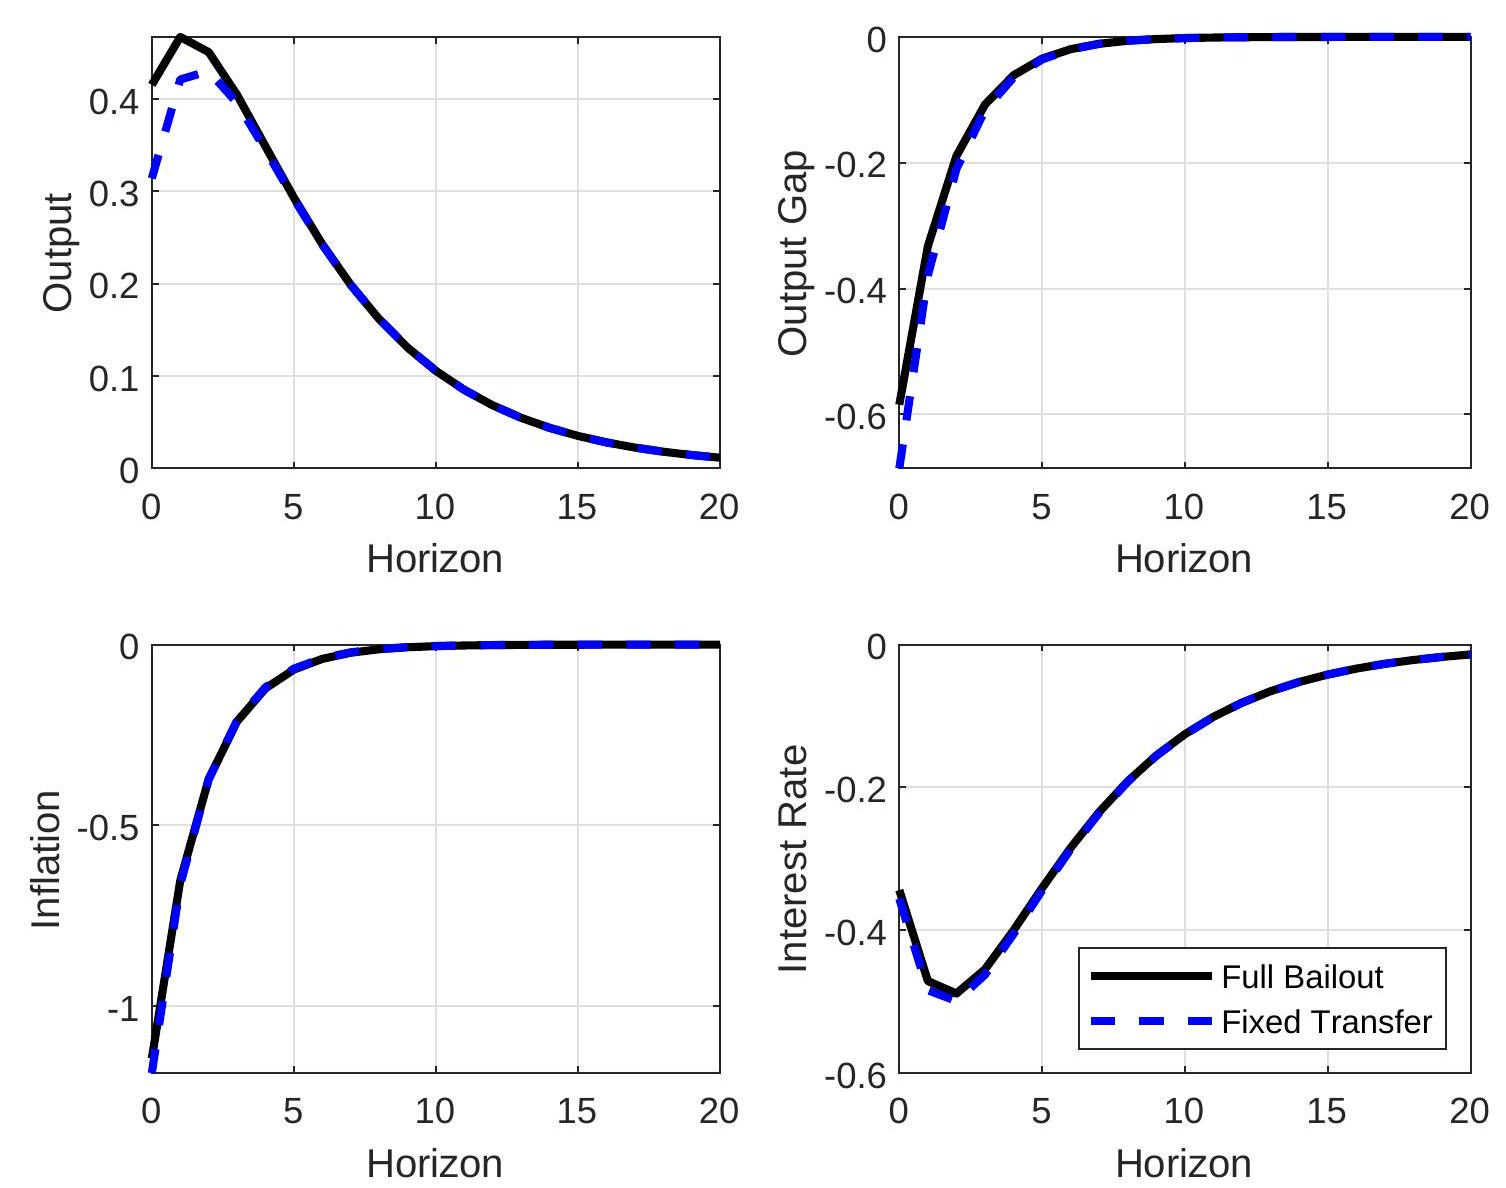
\includegraphics[max width=\textwidth, center]{2024_12_20_23d1456f4ac472ebd83dg-11}

Notes: Black solid lines: IRFs to a one percentage point shock to potential output in the baseline four equation model. Output and the output gap are expressed in percentage points, while the responses of inflation and the short term interest rate are expressed in annualized percentage points. Blue dashed lines: IRFs to the same-sized natural rate shock in the four equation model where there is no full bailout from parent to child.

Figure F.2: IRFs to Policy Shock, Fixed vs. Full Bailout\\
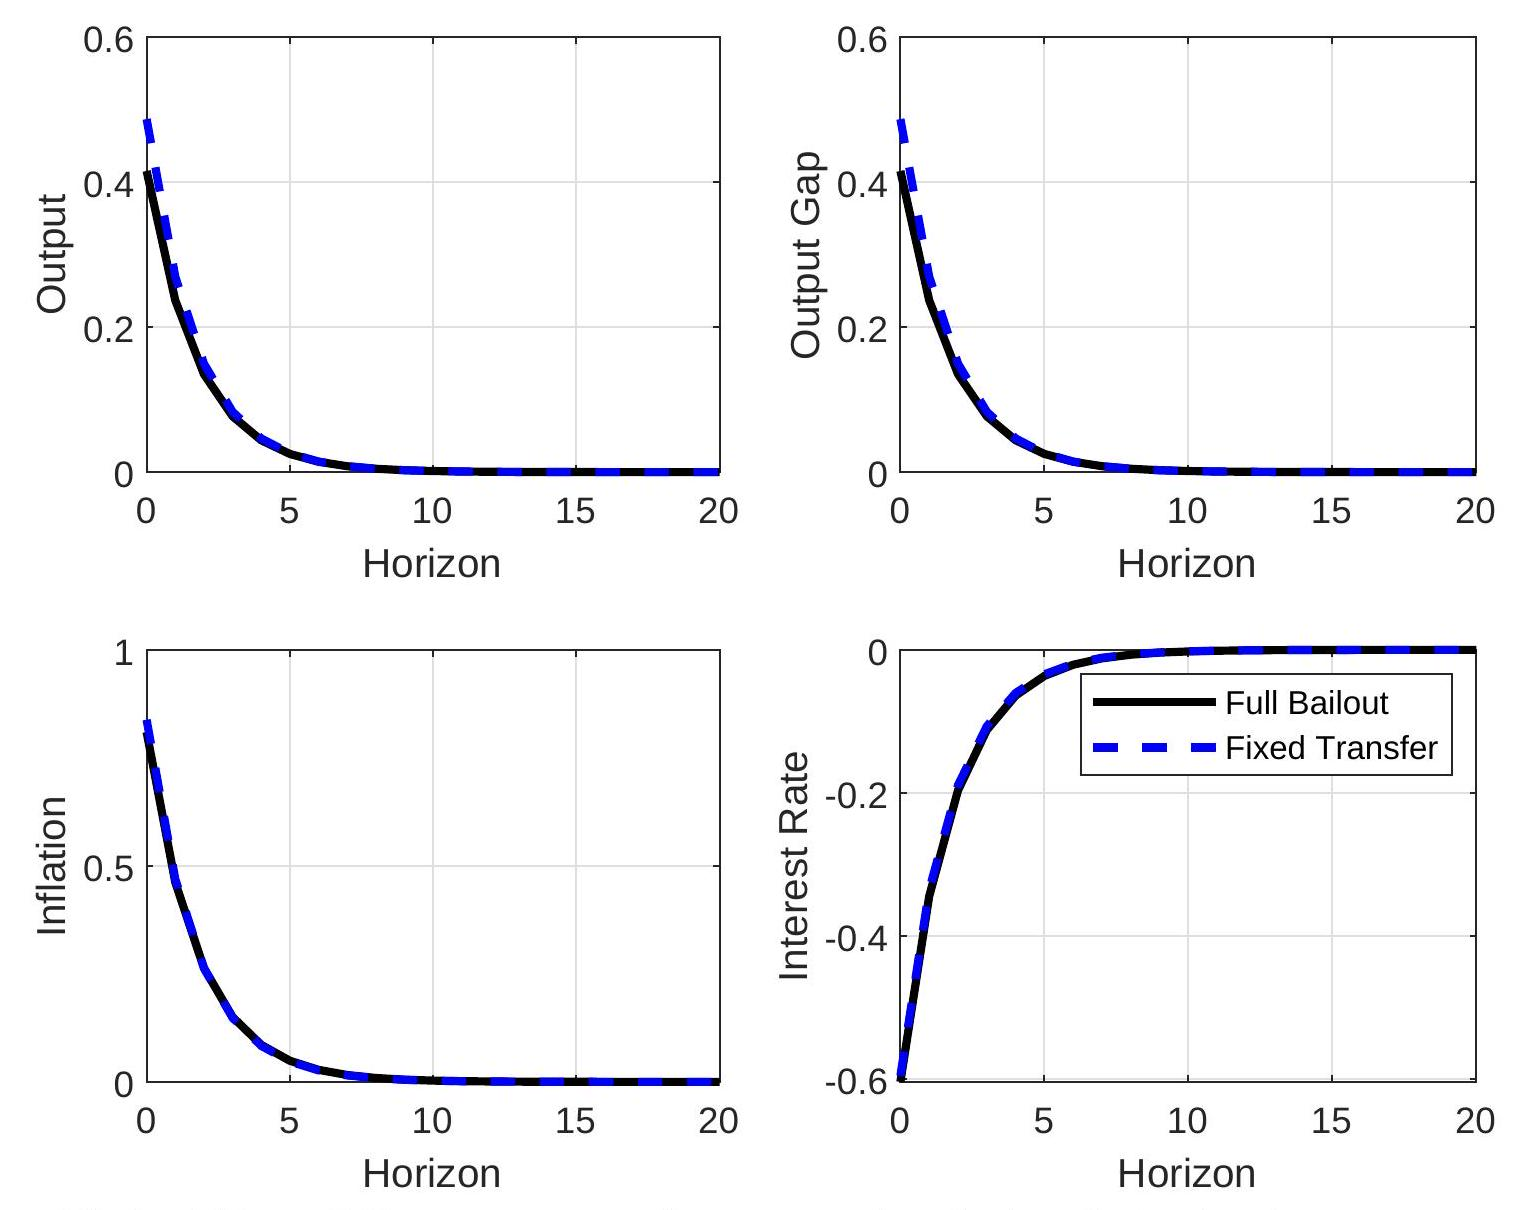
\includegraphics[max width=\textwidth, center]{2024_12_20_23d1456f4ac472ebd83dg-12}

Notes: Black solid lines: IRFs to a conventional monetary policy shock in the baseline four equation model. The size and sign of the shock are chosen to generate the same impact response of output as in Figure F.1. Output and the output gap are expressed in percentage points, while the responses of inflation and the short term interest rate are expressed in annualized percentage points. Blue dashed lines: IRFs to the same-sized policy shock in the four equation model where there is no full bailout from parent to child.

In the case of natural rate and monetary policy shocks, the differences for the responses of aggregate output, inflation, and the interest rate with or without the full bailout assumption are inconsequential. In comparison to our baseline model, output reacts slightly less to a natural rate shock on impact without the full bailout assumption; it reacts slightly more to a monetary policy shock without the full bailout assumption.

Figure F.3: IRFs to Credit/QE Shock, Fixed vs. Full Bailout\\
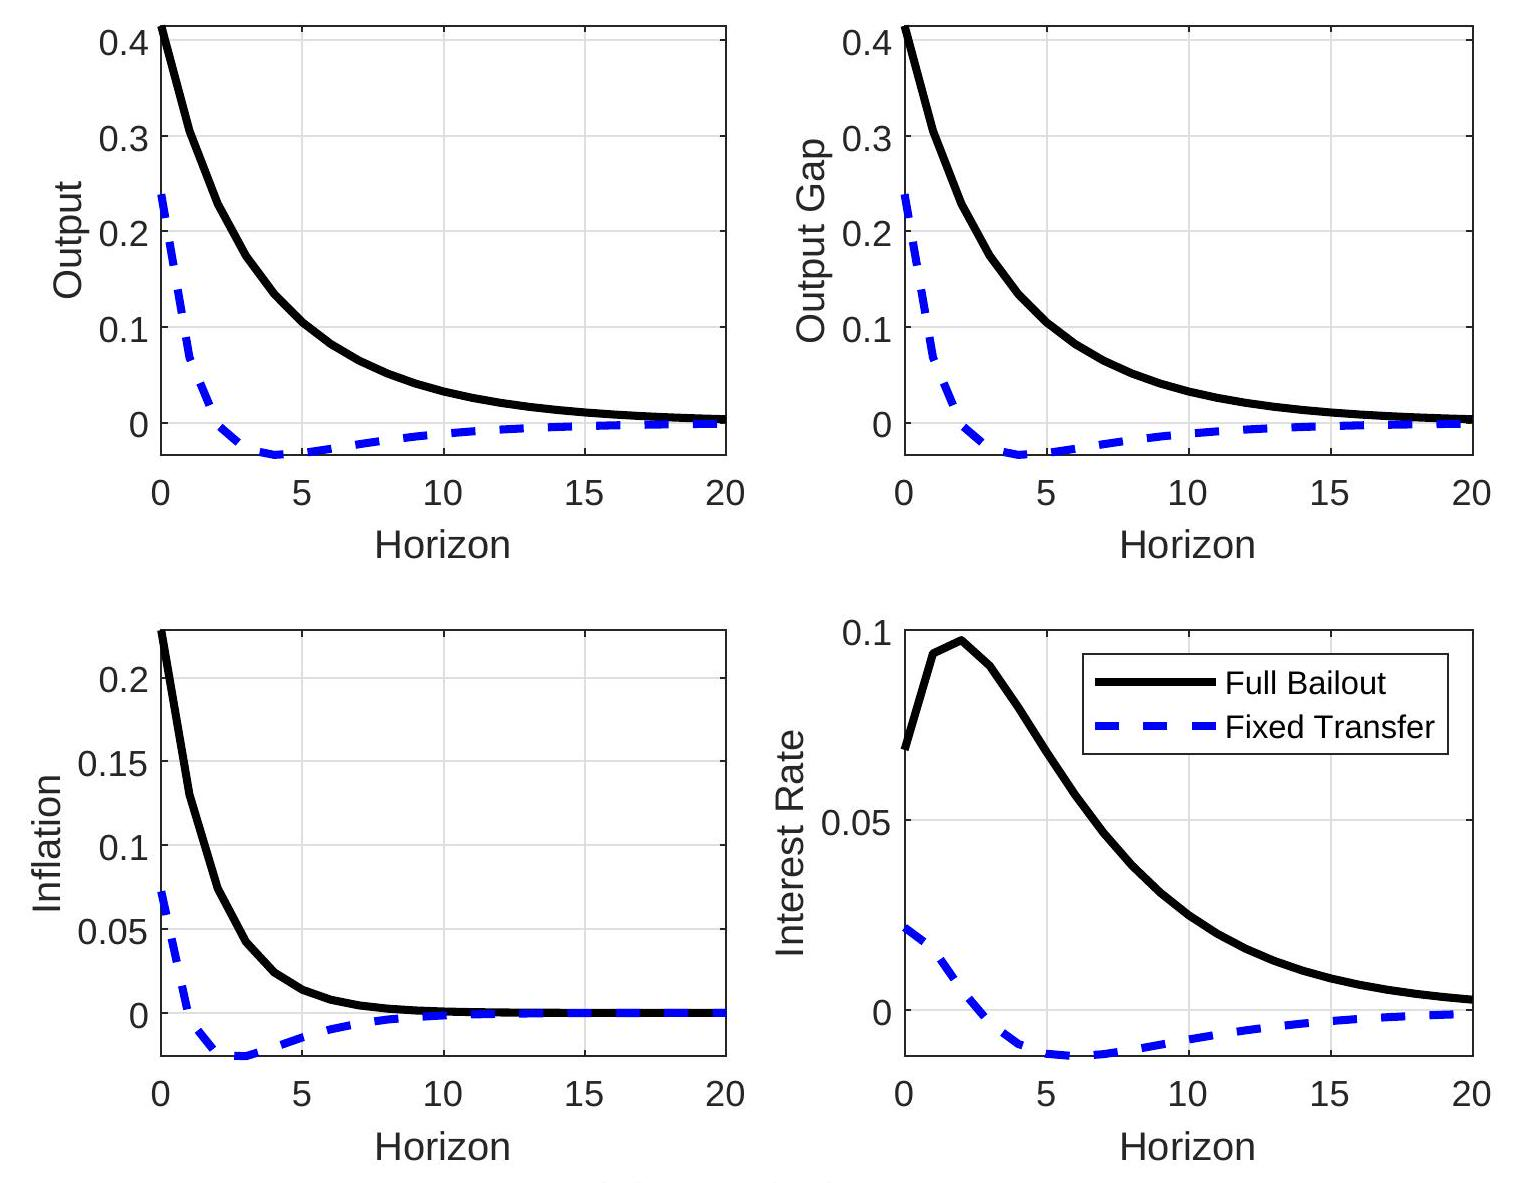
\includegraphics[max width=\textwidth, center]{2024_12_20_23d1456f4ac472ebd83dg-13}

Notes: Black solid lines: IRFs to a credit $\left(\theta_{t}\right)$ or QE $\left(q e_{t}\right)$ shock in the baseline four equation model. The size and sign of the shocks are chosen to generate the same impact response of output as in Figure F.1. Because the QE and credit shock only differ according to scale in the linearized model (i.e. $\bar{b}^{F I} \neq \bar{b}^{c b}$ ) and the AR parameters are the same, the normalized impulse responses are identical. Output and the output gap are expressed in percentage points, while the responses of inflation and the short term interest rate are expressed in annualized percentage points. Blue dashed lines: IRFs to the same-sized credit/QE shock in the four equation model where there is no full bailout from parent to child.

Quantitatively, differences are somewhat more noticeable when it comes to a credit or QE shock. Compared to the baseline model with the full bailout assumption, output and inflation react less on impact to a credit/QE shock when there is a fixed transfer. The responses are also less persistent. But qualitatively, they are in-line with our baseline model.

\section*{F. 2 Parameterization of $z$}
Our linearized four equation model differs from the standard NK model via the parameter $z$; when $z=0$, the model is equivalent to the standard three equation model. In this subsection, we show impulse responses to natural rate, monetary policy, and credit market shocks for different values of $z$. Responses with our baseline value of $z=0.33$ are depicted via solid black lines; we also show responses when $z=0.167$ (dotted black lines) and when $z=0.67$\\
(dashed black lines). For point of comparison, the blue dashed lines shows responses in the three equation model $(z=0)$.

In response to all three shocks, the bigger $z$ is, the more the responses differ from the conventional three equation model. Relative to our baseline case $(z=0.33)$, the impulse responses with $z=0.167$ or $z=0.667$ are not very wildly different.

Figure F.4: IRFs to Shock to Potential Output, Different Values of $z$\\
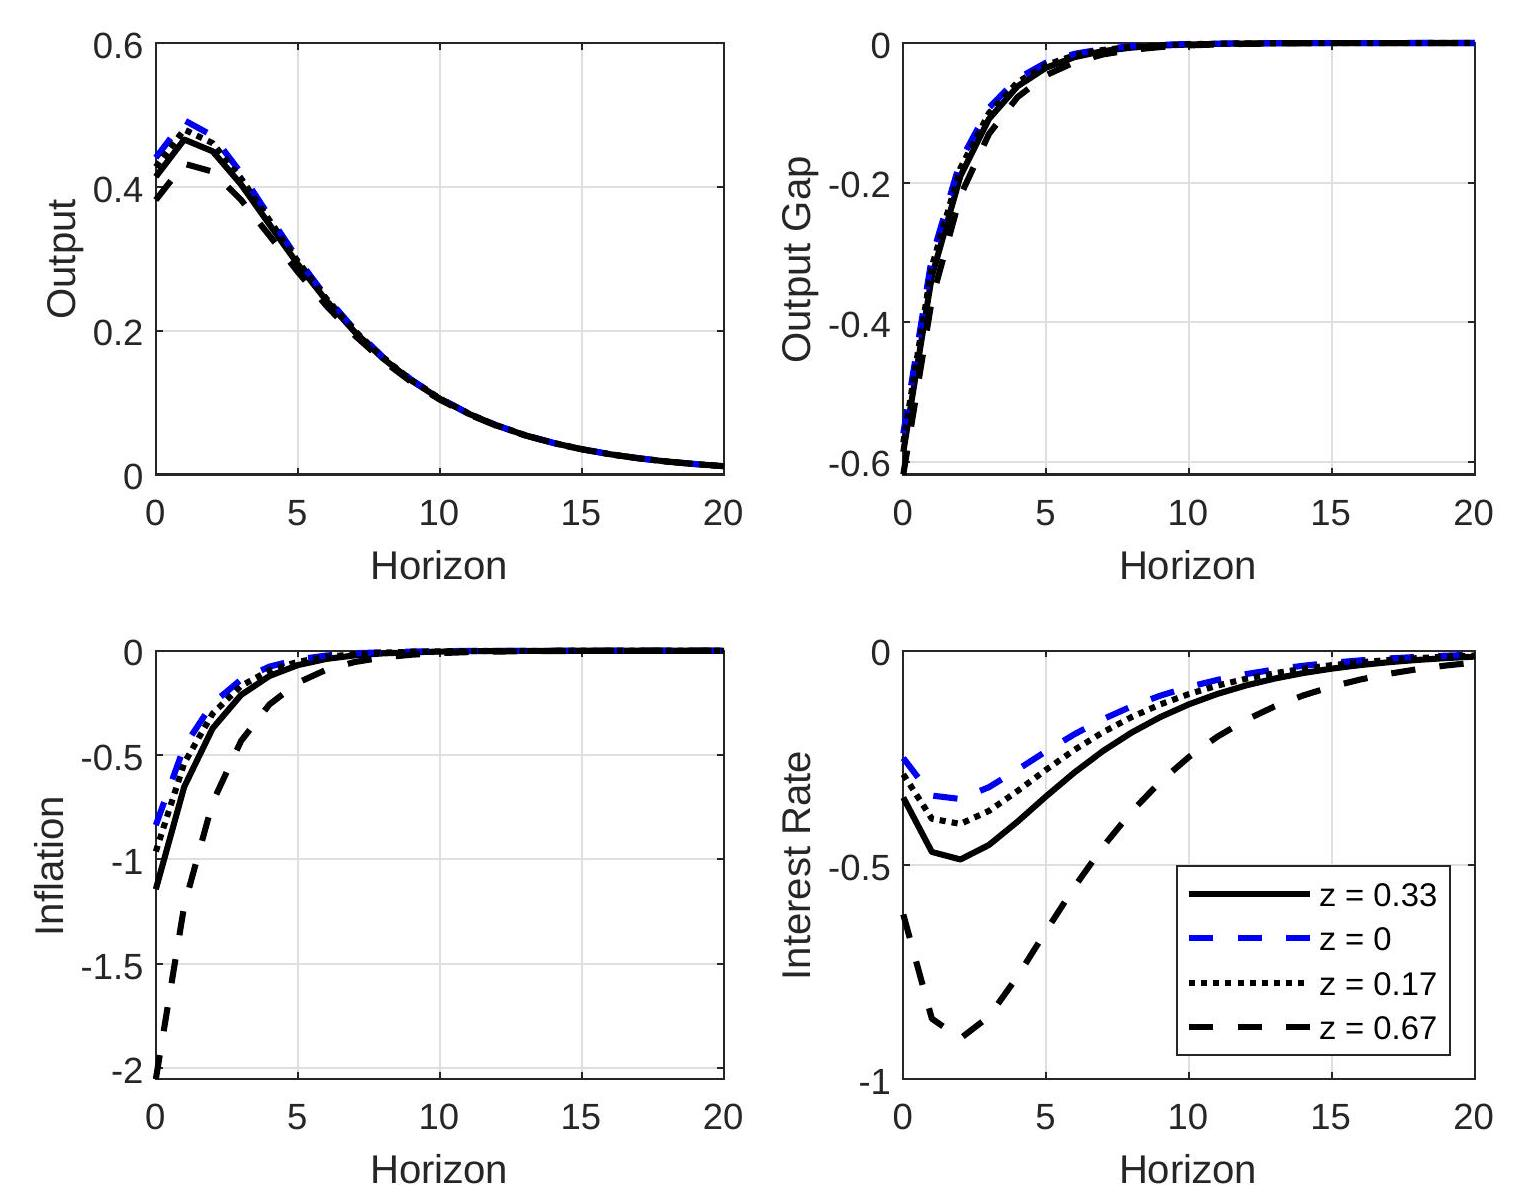
\includegraphics[max width=\textwidth, center]{2024_12_20_23d1456f4ac472ebd83dg-14}

Notes: Black solid lines: IRFs to a one percentage point shock to potential output in the baseline four equation model with $z=0.33$. Output and the output gap are expressed in percentage points, while the responses of inflation and the short term interest rate are expressed in annualized percentage points. Blue dashed lines: IRFs to the same-sized natural rate shock in the three equation model (equivalent to the four equation model with $z=0$ ). Black dotted lines: responses in the four equation model with $z=0.167$. Black dashed lines: responses in the four equation model with $z=0.667$.

Figure F.5: IRFs to Shock to Policy Shock, Different Values of $z$\\
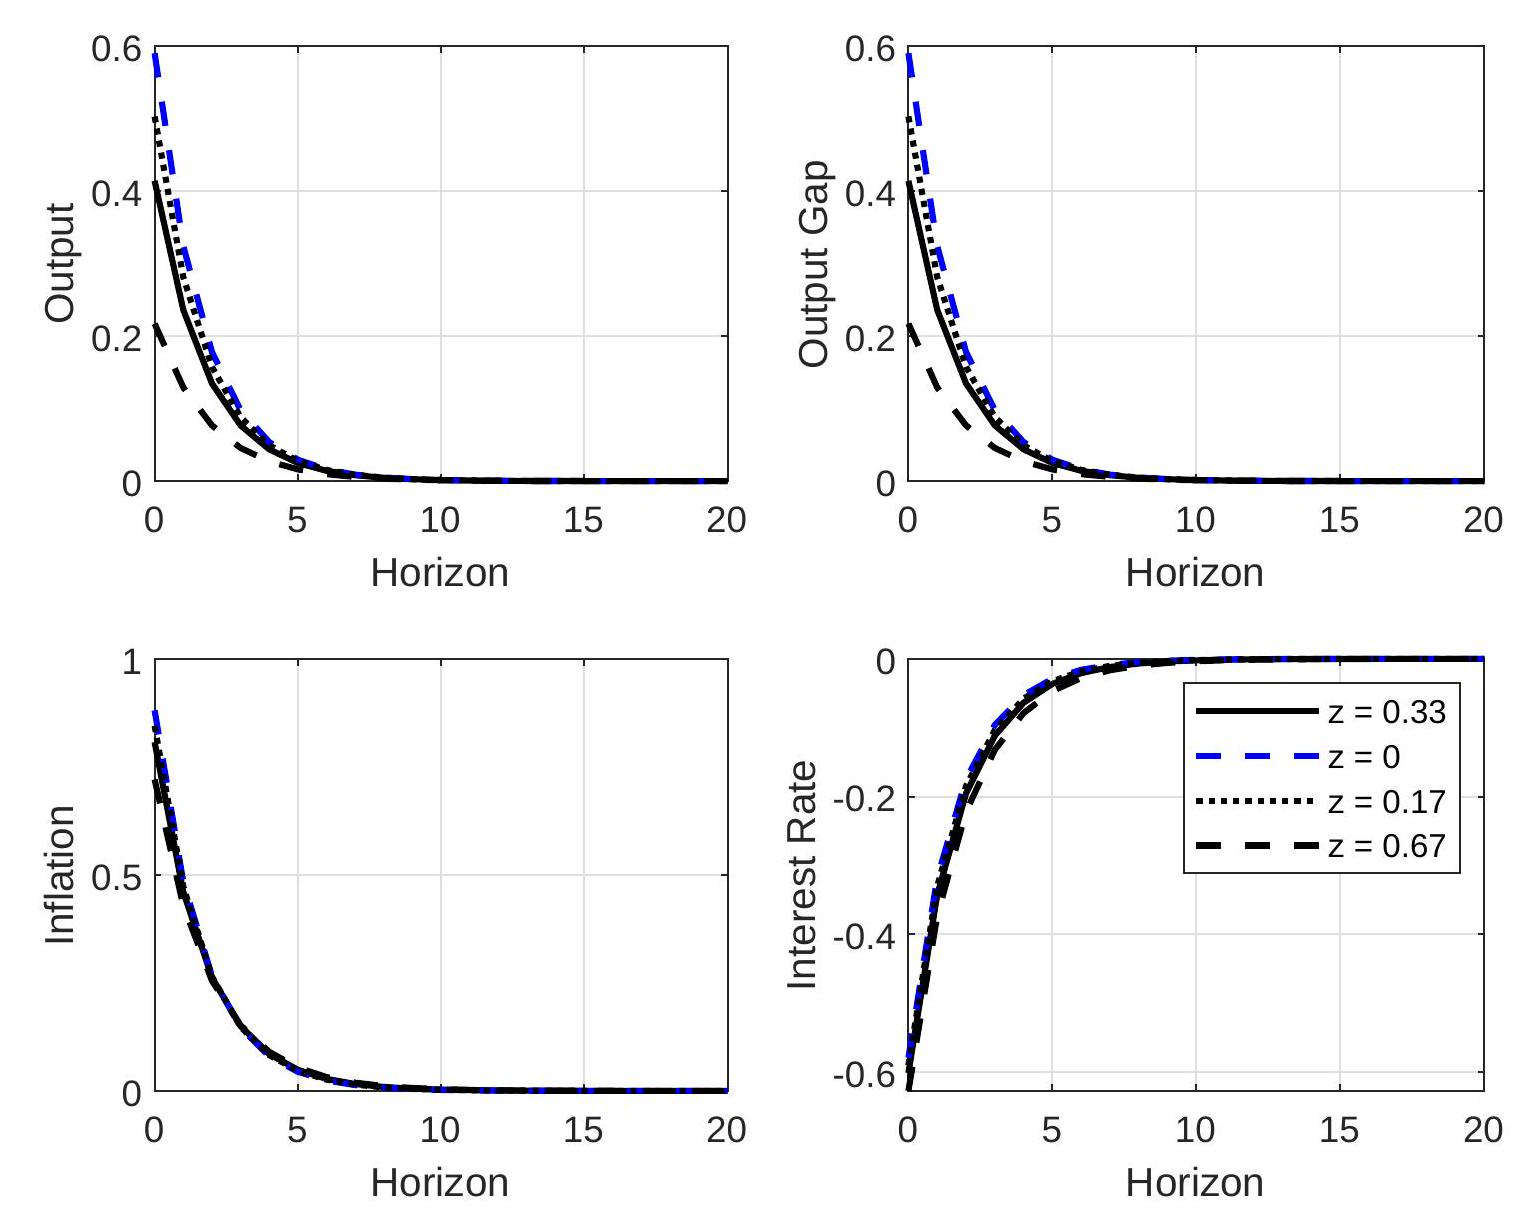
\includegraphics[max width=\textwidth, center]{2024_12_20_23d1456f4ac472ebd83dg-15}

Notes: Black solid lines: IRFs to a conventional monetary policy shock in the baseline four equation model with $z=0.33$. The size and sign of the shocks are chosen to generate the same impact response of output as in Figure F. 4 when $z=0.33$. Output and the output gap are expressed in percentage points, while the responses of inflation and the short term interest rate are expressed in annualized percentage points. Blue dashed lines: IRFs to the same-sized natural rate shock in the three equation model (equivalent to the four equation model with $z=0$ ). Black dotted lines: responses in the four equation model with $z=0.167$. Black dashed lines: responses in the four equation model with $z=0.667$.

Figure F.6: IRFs to Shock to Credit/QE Shock, Different Values of $z$\\
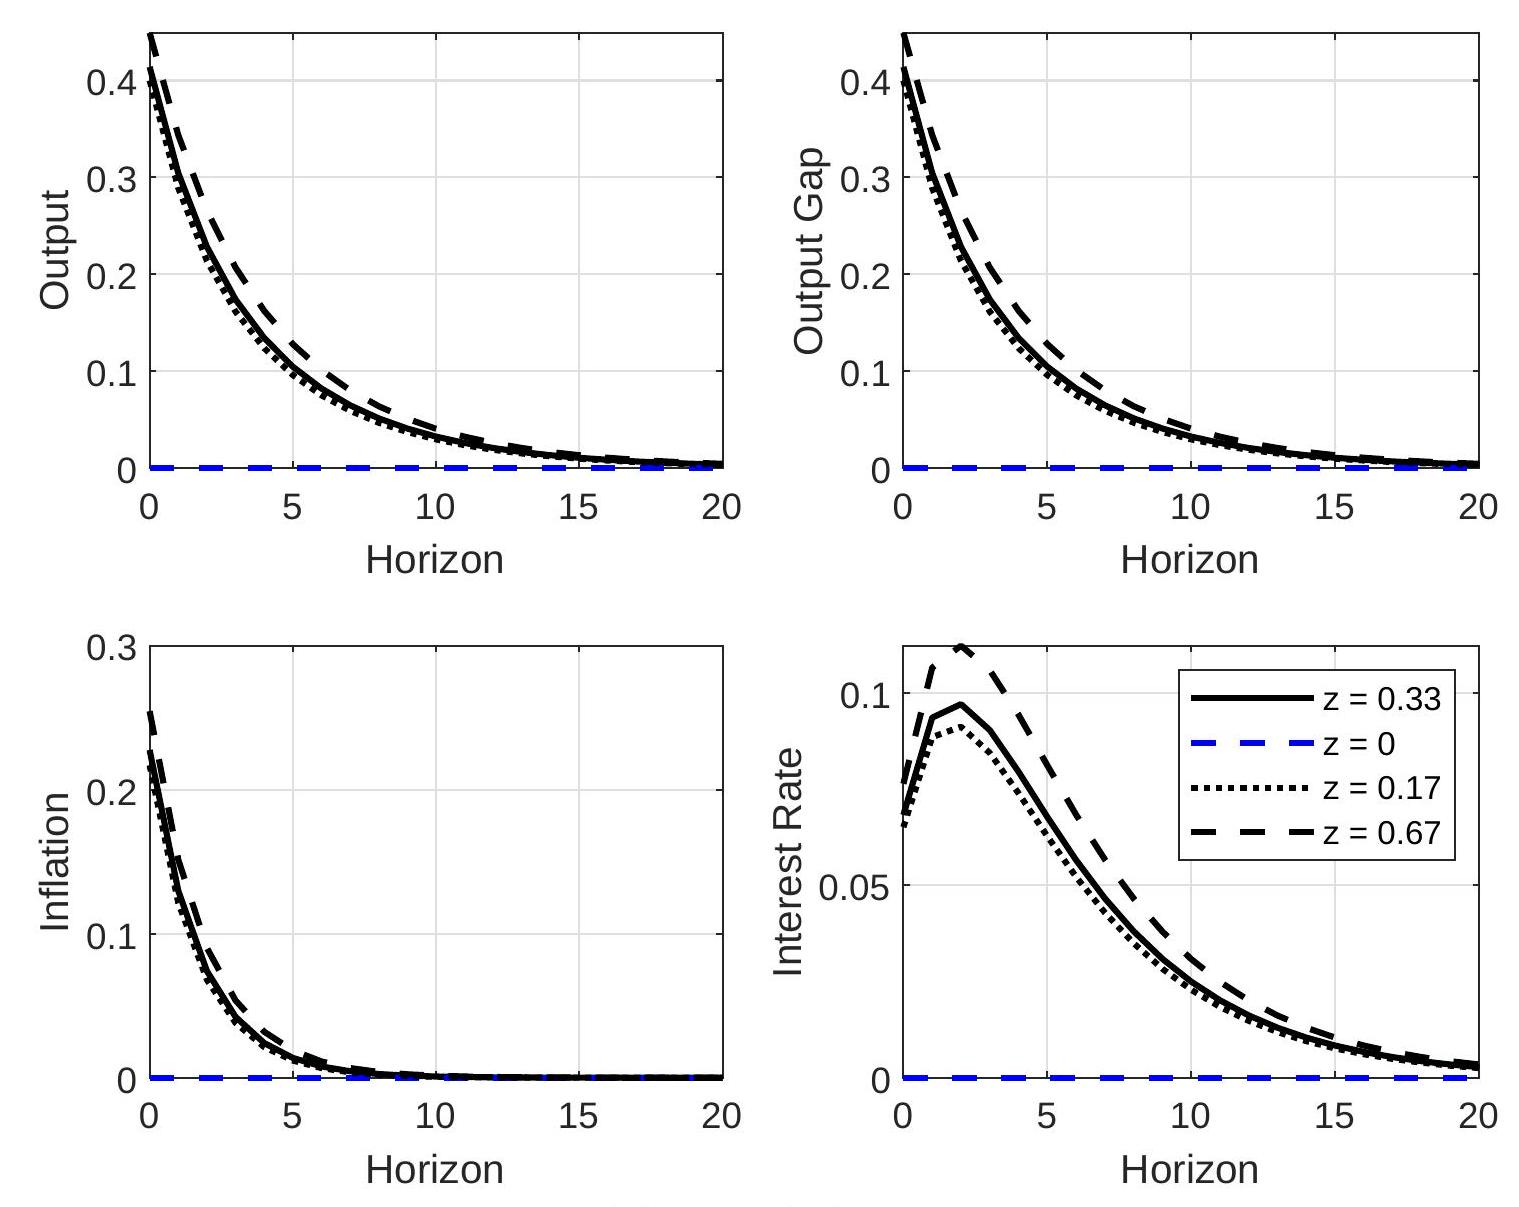
\includegraphics[max width=\textwidth, center]{2024_12_20_23d1456f4ac472ebd83dg-16}

Notes: Black solid lines: IRFs to a credit $\left(\theta_{t}\right)$ or QE $\left(q e_{t}\right)$ shock in the baseline four equation model with $z=0.33$. The size and sign of the shocks are chosen to generate the same impact response of output as in Figure F. 4 when $z=0.33$. Because the QE and credit shock only differ according to scale in the linearized model (i.e. $\bar{b}^{F I} \neq \bar{b}^{c b}$ ) and the AR parameters are the same, the normalized impulse responses are identical. Output and the output gap are expressed in percentage points, while the responses of inflation and the short term interest rate are expressed in annualized percentage points. Blue dashed lines: IRFs to the same-sized natural rate shock in the four equation model where there is no full bailout from parent to child.

\section*{G Optimal Monetary Policy}
We consider optimal monetary policy under discretion. The central bank's objective function is to pick instruments, $r_{t}^{s}$ and $q e_{t}$, and endogenous variables, $\pi_{t}$ and $x_{t}$, to minimize (3.1) subject to the IS equation, (2.1), the Phillips Curve, (2.2), a ZLB constraint on the policy rate, and a potential constraint on the use of balance sheet policies. Formally:\\
\begin{gather*}
\min _{r_{t}^{s}, q e_{t}, \pi_{t}, x_{t}} \mu x_{t}^{2}+\pi_{t}^{2} \\
\text { s.t. } \\
x_{t}=\mathbb{E}_{t} x_{t+1}-\frac{1-z}{\sigma}\left(r_{t}^{s}-\mathbb{E}_{t} \pi_{t+1}-r_{t}^{*}\right)-z\left[\bar{b}^{F I}\left(\mathbb{E}_{t} \theta_{t+1}-\theta_{t}\right)+\bar{b}^{c b}\left(\mathbb{E}_{t} q e_{t+1}-q e_{t}\right)\right], \tag{G.1}
\end{gather*}\\
\begin{gather*}
\pi_{t}=\gamma \zeta x_{t}-\frac{z \gamma \sigma}{1-z}\left[\bar{b}^{F I} \theta_{t}+\bar{b}^{c b} q e_{t}\right]+\beta \mathbb{E}_{t} \pi_{t+1}  \tag{G.2}\\
r_{t}^{s}=0  \tag{G.3}\\
q e_{t}=0 \tag{G.4}
\end{gather*}\\
(G.3) only holds when the policy rate is constrained by the ZLB (i.e. the policy rate is fixed), as in Section 3.2, while (G.4) only binds when QE is unavailable, as in Section 3.3. In solving the problem under discretion, the policymaker treats expectations of all future variables as given.

A Lagrangian is:

\begin{equation*}
\begin{aligned}
\mathbb{L}=\mu x_{t}^{2}+\pi_{t}^{2}+\lambda_{1, t} & \left(x_{t}-\mathbb{E}_{t} x_{t+1}+\frac{1-z}{\sigma}\left(r_{t}^{s}-\mathbb{E}_{t} \pi_{t+1}-r_{t}^{*}\right)+z\left[\bar{b}^{F I}\left(\mathbb{E}_{t} \theta_{t+1}-\theta_{t}\right)+\bar{b}^{c b}\left(\mathbb{E}_{t} q e_{t+1}-q e_{t}\right)\right]\right) \\
& +\lambda_{2, t}\left(\pi_{t}-\gamma \zeta x_{t}+\frac{z \gamma \sigma}{1-z}\left[\bar{b}^{F I} \theta_{t}+\bar{b}^{c b} q e_{t}\right]-\beta \mathbb{E}_{t} \pi_{t+1}\right)-\lambda_{3, t} r_{t}^{s}-\lambda_{4, t} q e_{t} .
\end{aligned}
\end{equation*}

The first order conditions are:\\
\begin{gather*}
\frac{\partial \mathbb{L}}{\partial r_{t}^{s}}=\lambda_{1, t} \frac{1-z}{\sigma}-\lambda_{3, t}=0  \tag{G.5}\\
\frac{\partial \mathbb{L}}{\partial q e_{t}}=-\lambda_{1, t} z \bar{b}^{c b}+\lambda_{2, t} \frac{z \gamma \sigma \bar{b}^{c b}}{1-z}-\lambda_{4, t}=0  \tag{G.6}\\
\frac{\partial \mathbb{L}}{\partial \pi_{t}}=2 \pi_{t}+\lambda_{2, t}=0  \tag{G.7}\\
\frac{\partial \mathbb{L}}{\partial x_{t}}=2 \mu x_{t}+\lambda_{1, t}-\gamma \zeta \lambda_{2, t}=0 \tag{G.8}
\end{gather*}

\section*{G. 1 Both Instruments Available}
When both instruments are available, we have $\lambda_{3, t}=\lambda_{4, t}=0$. From (G.5), this means that $\lambda_{1, t}=0$. But then from (G.6), $\lambda_{1, t}=\lambda_{4, t}=0$ implies that $\lambda_{2, t}=0$. But then (G.7) then requires that $\pi_{t}=0$. Then, from (G.8), we see that $x_{t}=0$.

\section*{G.1.1 Proof of Theorem 1}
The theorem can be proved by contradiction. Suppose first we can achieve $x_{t}=\pi_{t}=0$ with $q e_{t}=0$ for all $t$. Then the Phillips curve may then be written as:

\begin{equation*}
0=-\frac{z \gamma \sigma}{1-z} \bar{b}^{F I} \theta_{t} \tag{G.9}
\end{equation*}

which does not hold unless $\theta_{t}=0$, which contradicts the assumption. Hence, there is a contradiction.

Second, suppose we can achieve $x_{t}=\pi_{t}=\mathbb{E}_{t} x_{t+1}=\mathbb{E}_{t} \pi_{t+1}=0$ with $r_{t}^{s}=0$ for all $t$.

Then the Phillips curve becomes

\begin{equation*}
0=\frac{z \gamma \sigma}{1-z}\left[\bar{b}^{F I} \theta_{t}+\bar{b}^{c b} q e_{t}\right] . \tag{G.10}
\end{equation*}

This requires

\begin{equation*}
q e_{t}=-\frac{\bar{b}^{F I}}{\bar{b}^{c b}} \theta_{t} . \tag{G.11}
\end{equation*}

Note that (G.11) is identical to the equilibrium path for $q e_{t}$ given in Proposition 2. With the policy rate fixed and the equilibrium path of QE given in this way, the IS curve becomes

\begin{equation*}
0=\frac{1-z}{\sigma} r_{t}^{*}-z\left[\bar{b}^{F I}\left(\mathbb{E}_{t} \theta_{t+1}-\theta_{t}\right)+\bar{b}^{c b}\left(\mathbb{E}_{t} q e_{t+1}-q e_{t}\right)\right] . \tag{G.12}
\end{equation*}

Further apply (G.11) on both $q e_{t}$ and $\mathbb{E}_{t} q e_{t+1}$. This implies

\begin{equation*}
0=\frac{1-z}{\sigma} r_{t}^{*} \tag{G.13}
\end{equation*}

which does not hold unless $z=1$ (which we have ruled out) or $r_{t}^{*}=0$ (which contradicts the assumption). Hence, we have another contradiction. -

\section*{G. 2 The ZLB}
\section*{G.2.1 First Order Condition}
Next, suppose that the ZLB binds, so $\lambda_{3, t} \geq 0$, but QE is available, so $\lambda_{4, t}=0$. We will have $\lambda_{1, t}>0$. We can solve for $\lambda_{1, t}$ in terms of $\lambda_{2, t}$ from (G.6):

\begin{equation*}
\lambda_{1, t}=\frac{\gamma \sigma}{1-z} \lambda_{2, t} \tag{G.14}
\end{equation*}

Then, from (G.8), we have:

\begin{equation*}
\frac{2 \mu(1-z)}{\gamma \zeta(1-z)-\gamma \sigma} x_{t}=\lambda_{2, t} . \tag{G.15}
\end{equation*}

Plug (G.15) into (G.7):

\begin{equation*}
2 \pi_{t}+\frac{2 \mu(1-z)}{\gamma \zeta(1-z)-\gamma \sigma} x_{t}=0
\end{equation*}

Simplifying yields:

\begin{equation*}
\pi_{t}=-\frac{\mu(1-z)}{\gamma \zeta(1-z)-\gamma \sigma} x_{t} \tag{G.16}
\end{equation*}

as shown in the main text.

\section*{G.2.2 Proof of Proposition 2}
When the ZLB is binding, the IS curve becomes

\begin{equation*}
x_{t}=\mathbb{E}_{t} x_{t+1}-\frac{1-z}{\sigma}\left(-\mathbb{E}_{t} \pi_{t+1}-r_{t}^{*}\right)-z\left[\bar{b}^{F I}\left(\mathbb{E}_{t} \theta_{t+1}-\theta_{t}\right)+\bar{b}^{c b}\left(\mathbb{E}_{t} q e_{t+1}-q e_{t}\right)\right], \tag{G.17}
\end{equation*}

and the Phillips curve remains as (2.2). (3.4) holds and describes balance sheet policy, and the policy rate is fixed, i.e. $r_{t}^{s}=0$.

Guess

\begin{equation*}
\pi_{t}=\omega_{1} r_{t}^{*}+\omega_{3} \theta_{t}
\end{equation*}

then (3.4) implies

\begin{equation*}
x_{t}=-\frac{\gamma \zeta(1-z)-\gamma \sigma}{\mu(1-z)}\left(\omega_{1} r_{t}^{*}+\omega_{3} \theta_{t}\right) \equiv \omega_{2}\left(\omega_{1} r_{t}^{*}+\omega_{3} \theta_{t}\right) .
\end{equation*}

If in period $t+1$, the economy exits the ZLB, then both instruments are available, which implies $\pi_{t+1}=x_{t+1}=0$. If in period $t+1$, the economy is still at the ZLB, $\pi_{t+1}=$ $\omega_{1} r_{t+1}^{*}+\omega_{3} \theta_{t+1}, x_{t+1}=\omega_{2}\left(\omega_{1} r_{t+1}^{*}+\omega_{3} \theta_{t+1}\right)$. As a result,

\begin{equation*}
\begin{aligned}
& \mathbb{E}_{t} \pi_{t+1}=\alpha\left(\rho_{f} \omega_{1} r_{t}^{*}+\rho_{\theta} \omega_{3} \theta_{t}\right) \\
& \mathbb{E}_{t} x_{t+1}=\alpha \omega_{2}\left(\rho_{f} \omega_{1} r_{t}^{*}+\rho_{\theta} \omega_{3} \theta_{t}\right)
\end{aligned}
\end{equation*}

We also guess the equilibrium path of QE is:

\begin{equation*}
q e_{t}=\tau r_{t}^{*}+\omega_{4} \theta_{t}
\end{equation*}

If in period $t+1$, the economy exits the ZLB, then everything goes back to the unconstrained case: $q e_{t+1}=-\frac{\hat{b}^{F I}}{b^{c b}} \theta_{t+1}$. Otherwise, $q e_{t+1}=\tau r_{t+1}^{*}+\omega_{4} \theta_{t+1}$. Then,

\begin{equation*}
\mathbb{E}_{t} q e_{t+1}=\alpha \rho_{f} \tau r_{t}^{*}+\alpha \rho_{\theta} \omega_{4} \theta_{t}-(1-\alpha) \rho_{\theta} \frac{\bar{b}^{F I}}{\bar{b} c b} \theta_{t}
\end{equation*}

Plugging the guesses into (2.2) and (G.17), we have:\\
\begin{align*}
& \omega_{1} r_{t}^{*}+\omega_{3} \theta_{t}=\gamma \zeta \omega_{2}\left(\omega_{1} r_{t}^{*}+\omega_{3} \theta_{t}\right)-\frac{z \gamma \sigma}{1-z}\left[\left(\bar{b}^{F I}+\bar{b}^{c b} \omega_{4}\right) \theta_{t}+\bar{b}^{c b} \tau r_{t}^{*}\right]+\beta \alpha\left(\rho_{f} \omega_{1} r_{t}^{*}+\rho_{\theta} \omega_{3} \theta_{t}\right),  \tag{G.18}\\
& \omega_{2}\left(\omega_{1} r_{t}^{*}+\omega_{3} \theta_{t}\right)=\alpha \omega_{2}\left(\rho_{f} \omega_{1} r_{t}^{*}+\rho_{\theta} \omega_{3} \theta_{t}\right)-\frac{1-z}{\sigma}\left[-\alpha\left(\rho_{f} \omega_{1} r_{t}^{*}+\rho_{\theta} \omega_{3} \theta_{t}\right)-r_{t}^{*}\right] \\
& -z \bar{b}^{F I}\left(\rho_{\theta}-1\right) \theta_{t}-z \bar{b}^{c b}\left[\alpha \rho_{\theta} \omega_{4}-(1-\alpha) \rho_{\theta} \frac{\bar{b}^{F I}}{\bar{b}^{c b}}-\omega_{4}\right] \theta_{t} \\
& -z \bar{b}^{c b}\left(\alpha \rho_{f}-1\right) \tau r_{t}^{*} . \tag{G.19}
\end{align*}

Matching coefficients, we have the following system of equations:\\
\begin{align*}
\omega_{1} & =\gamma \zeta \omega_{2} \omega_{1}-\frac{z \gamma \sigma}{1-z} \bar{b}^{c b} \tau+\beta \alpha \rho_{f} \omega_{1}  \tag{G.20}\\
\omega_{2} \omega_{1} & =\alpha \omega_{2} \rho_{f} \omega_{1}+\frac{1-z}{\sigma}\left(\alpha \rho_{f} \omega_{1}+1\right)-z \bar{b}^{c b}\left(\alpha \rho_{f}-1\right) \tau  \tag{G.21}\\
\omega_{3} & =\gamma \zeta \omega_{2} \omega_{3}-\frac{z \gamma \sigma}{1-z}\left(\bar{b}^{F I}+\bar{b}^{c b} \omega_{4}\right)+\beta \alpha \rho_{\theta} \omega_{3}  \tag{G.22}\\
\omega_{2} \omega_{3} & =\alpha \omega_{2} \rho_{\theta} \omega_{3}+\frac{1-z}{\sigma} \alpha \rho_{\theta} \omega_{3}-z \bar{b}^{F I}\left(\rho_{\theta}-1\right)-z \bar{b}^{c b}\left[\alpha \rho_{\theta} \omega_{4}-(1-\alpha) \rho_{\theta} \frac{\bar{b} \bar{b}}{\overline{b I}}-\omega \alpha\right] . \tag{23}
\end{align*}

Solve $\tau$ as a function of $\omega_{1}$ in the first two equations

\begin{equation*}
\begin{aligned}
\tau & =\frac{(1-z)\left(\gamma \zeta \omega_{2} \omega_{1}+\beta \alpha \rho_{f} \omega_{1}-\omega_{1}\right)}{\bar{b}^{c b} z \gamma \sigma} \\
\tau & =\frac{\alpha \omega_{2} \rho_{f} \omega_{1}+\frac{1-z}{\sigma}\left(\alpha \rho_{f} \omega_{1}+1\right)-\omega_{2} \omega_{1}}{z \bar{b}^{c b}\left(\alpha \rho_{f}-1\right)}
\end{aligned}
\end{equation*}

The first equation is the same as (3.10). Then,

\begin{equation*}
\frac{\alpha \omega_{2} \rho_{f} \omega_{1}+\frac{1-z}{\sigma}\left(\alpha \rho_{f} \omega_{1}+1\right)-\omega_{2} \omega_{1}}{z \bar{b}^{c b}\left(\alpha \rho_{f}-1\right)}=\frac{(1-z)\left(\gamma \zeta \omega_{2} \omega_{1}+\beta \alpha \rho_{f} \omega_{1}-\omega_{1}\right)}{\bar{b}^{c b} z \gamma \sigma}
\end{equation*}

Simplify, we get

\begin{equation*}
\omega_{1}=\frac{\gamma(1-z)}{\left(\alpha \rho_{f}-1\right)(1-z)\left(\gamma \zeta \omega_{2}+\beta \alpha \rho_{f}-1\right)-\gamma \sigma \alpha \omega_{2} \rho_{f}-\gamma(1-z) \alpha \rho_{f}+\gamma \sigma \omega_{2}}
\end{equation*}

This is the same as (3.8).\\
Next, simplify (G.23)

\begin{equation*}
\omega_{2} \omega_{3}=\alpha \omega_{2} \rho_{\theta} \omega_{3}+\frac{1-z}{\sigma} \alpha \rho_{\theta} \omega_{3}+z\left(1-\alpha \rho_{\theta}\right)\left(\bar{b}^{F I}+\bar{b}^{c b} \omega_{4}\right)
\end{equation*}

Therefore,

\begin{equation*}
\bar{b}^{F I}+\bar{b}^{c b} \omega_{4}=\frac{\omega_{2}-\alpha \omega_{2} \rho_{\theta}-\frac{1-z}{\sigma} \alpha \rho_{\theta}}{z\left(1-\alpha \rho_{\theta}\right)} \omega_{3} \tag{G.24}
\end{equation*}

Similarly, rearrange (G.22)

\begin{equation*}
\bar{b}^{F I}+\bar{b}^{c b} \omega_{4}=\left(\gamma \zeta \omega_{2}+\beta \alpha \rho_{\theta}-1\right) \frac{1-z}{z \gamma \sigma} \omega_{3} \tag{G.25}
\end{equation*}

Combining (G.24)-(G.25),

\begin{equation*}
\left(\frac{\omega_{2}-\alpha \omega_{2} \rho_{\theta}-\frac{1-z}{\sigma} \alpha \rho_{\theta}}{z\left(1-\alpha \rho_{\theta}\right)}-\left(\gamma \zeta \omega_{2}+\beta \alpha \rho_{\theta}-1\right) \frac{1-z}{z \gamma \sigma}\right) \omega_{3}=0
\end{equation*}

This has to hold for any parameter specification. Therefore,

\begin{equation*}
\omega_{3}=0
\end{equation*}

Plug back to (G.24), we get

\begin{equation*}
\omega_{4}=-\frac{\bar{b}^{F I}}{\bar{b}^{c b}} .
\end{equation*}

\section*{G. 3 No QE Available}
\section*{G.3.1 First Order Condition}
When QE is unavailable, we have $\lambda_{4, t}>0$, but $\lambda_{3, t}=0$. The later implies from (G.5) that $\lambda_{1, t}=0$. From (G.7), we have:

\begin{equation*}
\lambda_{2, t}=-2 \pi_{t} . \tag{G.26}
\end{equation*}

Plugging into (G.8), we have:

\begin{equation*}
2 \mu x_{t}+2 \gamma \zeta \pi_{t}=0 \tag{G.27}
\end{equation*}

which implies:

\begin{equation*}
\pi_{t}=-\frac{\mu}{\gamma \zeta} x_{t} \tag{G.28}
\end{equation*}

as shown in the text.

\section*{G.3.2 Proof of Proposition 3}
When QE policy is not available, (3.11) holds, and $q e_{t}=0$. The IS Phillips curves can be written:

\begin{equation*}
x_{t}=\mathbb{E}_{t} x_{t+1}-\frac{1-z}{\sigma}\left(r_{t}^{s}-\mathbb{E}_{t} \pi_{t+1}-r_{t}^{*}\right)-z \bar{b}^{F I}\left(\mathbb{E}_{t} \theta_{t+1}-\theta_{t}\right), \tag{G.29}
\end{equation*}

and

\begin{equation*}
\pi_{t}=\gamma \zeta x_{t}-\frac{z \gamma \sigma}{1-z} \bar{b}^{F I} \theta_{t}+\beta \mathbb{E}_{t} \pi_{t+1} \tag{G.30}
\end{equation*}

Substitute (3.11) into (G.30)

\begin{equation*}
\pi_{t}=-\frac{\gamma^{2} \zeta^{2}}{\mu} \pi_{t}+\beta \mathbb{E}_{t} \pi_{t+1}-\frac{z \gamma \sigma}{1-z} \bar{b}^{F I} \theta_{t} \tag{G.31}
\end{equation*}

Solve the above equation forward, we have

\begin{equation*}
\pi_{t}=\varphi \theta_{t} \tag{G.32}
\end{equation*}

where

\begin{equation*}
\varphi=-\frac{\mu}{\gamma^{2} \zeta^{2}+\mu\left(1-\beta \rho_{\theta}\right)} \frac{z \gamma \sigma}{1-z} \bar{b}^{F I} . \tag{G.33}
\end{equation*}

Combining the solution for $\pi_{t}$ and (3.11), we obtain

\begin{equation*}
x_{t}=-\frac{\gamma \zeta}{\mu} \varphi \theta_{t} . \tag{G.34}
\end{equation*}

Plug the solutions for $\pi_{t}$ and $x_{t}$ into (G.29):

\begin{equation*}
r_{t}^{s}=r_{t}^{*}+\left[\rho_{\theta} \varphi+\frac{\sigma\left(1-\rho_{\theta}\right)}{1-z} \frac{\gamma \zeta}{\mu} \varphi+\frac{\left(1-\rho_{\theta}\right) \sigma z \bar{b}^{F I}}{1-z}\right] \theta_{t} \tag{G.35}
\end{equation*}

As a result,

\begin{equation*}
\eta=\rho_{\theta} \varphi+\frac{\sigma\left(1-\rho_{\theta}\right)}{1-z} \frac{\gamma \zeta}{\mu} \varphi+\frac{\left(1-\rho_{\theta}\right) \sigma z \bar{b}^{F I}}{1-z} \tag{G.36}
\end{equation*}

\section*{H Additional Results}
Figure H. 1 plots the optimal QE response to a natural rate shock, $\tau$, as a function of $\alpha$, which governs the expected duration of a ZLB episode. These results are discussed in Section 3.2 of the text.

Figure H.1: $\tau$ As a Function of ZLB Duration, $\alpha$\\
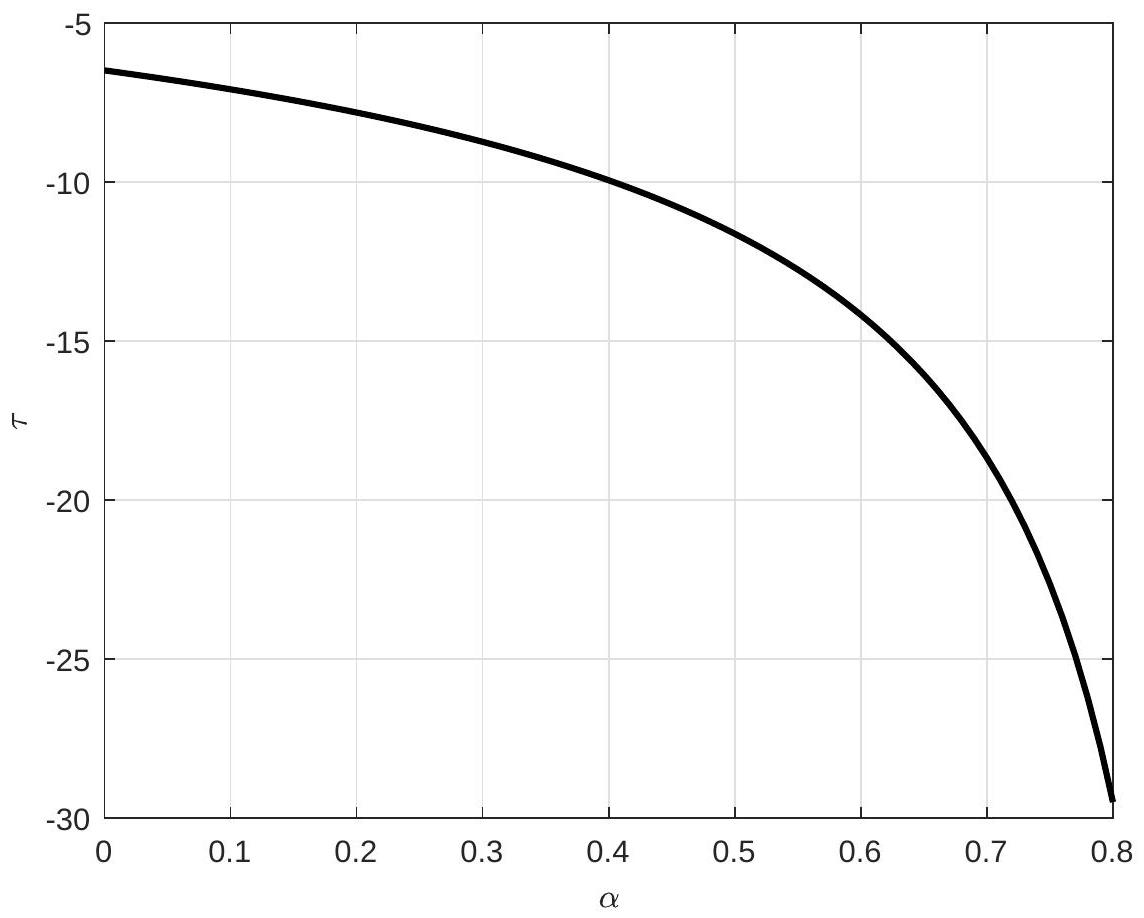
\includegraphics[max width=\textwidth, center]{2024_12_20_23d1456f4ac472ebd83dg-23}

Notes: This figure plots the response of QE to a natural rate shock under optimal policy when the ZLB binds for different values of $\alpha$. The expected duration of the ZLB is $1 /(1-\alpha)$, so higher values of $\alpha$ correspond to higher expected ZLB durations. The figure is generated assuming a value of $\mu=1$.

Figure H. 2 plots the optimal QE response to a natural rate shock, $\tau$, as a function of $\mu$, the relative weight the central bank attaches to the output gap. These results are discussed in Section 3.2 of the text.

Figure H.2: $\tau$ as a Function of $\mu$\\
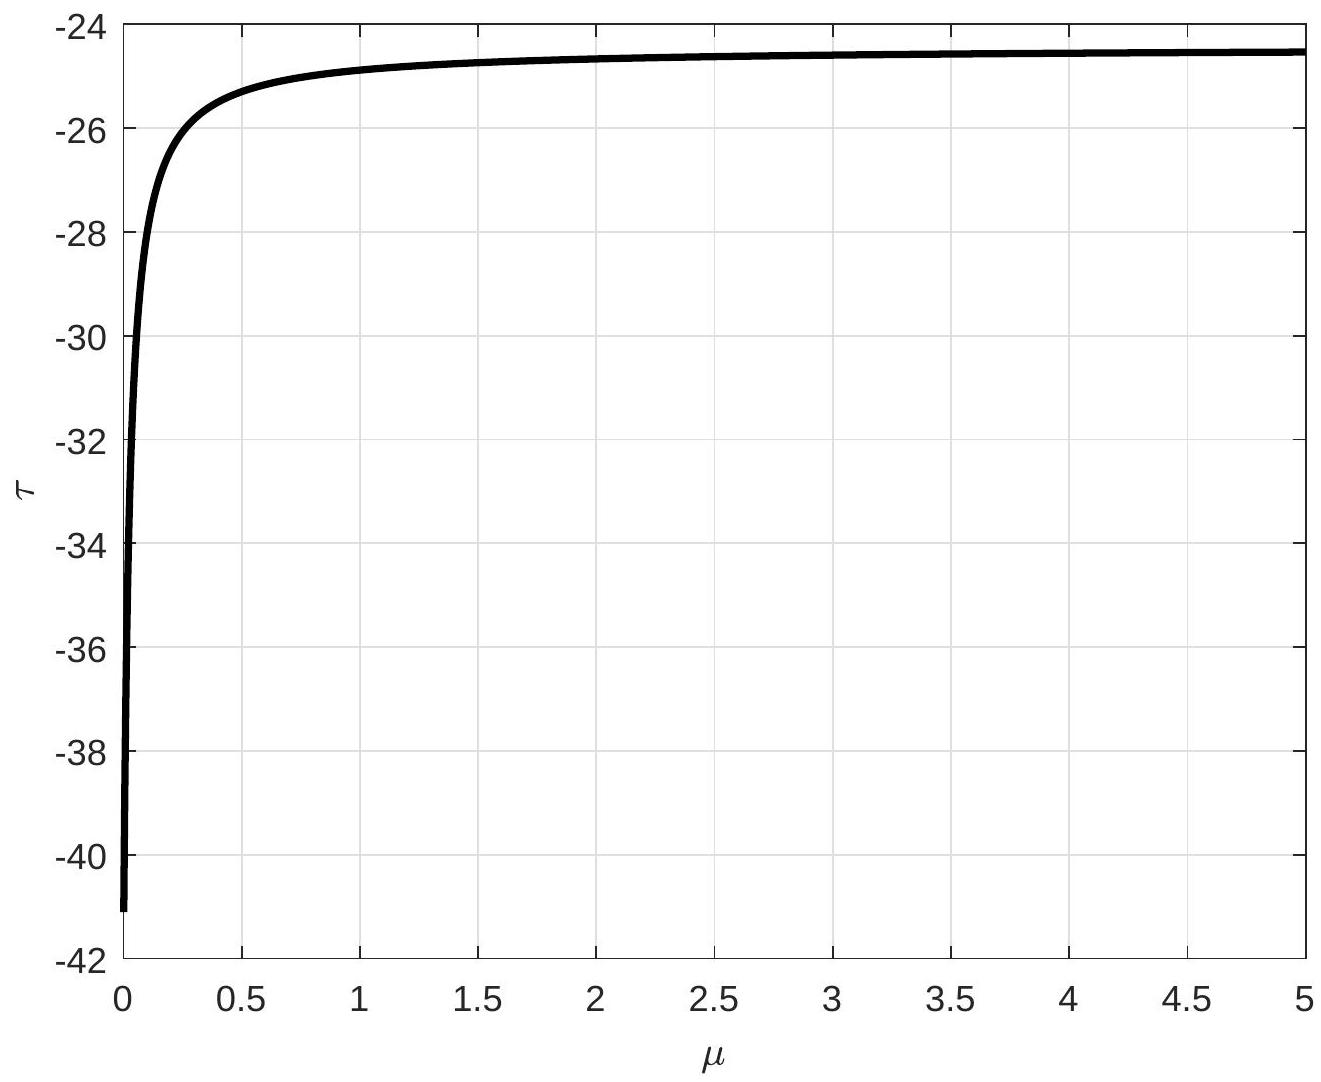
\includegraphics[max width=\textwidth, center]{2024_12_20_23d1456f4ac472ebd83dg-24}

Notes: This figure plots the response of QE to a natural rate shock under optimal policy when the ZLB binds, with $\alpha=3 / 4$, for different values of $\mu$, the welfare weight on the output gap.

Figure H. 3 plots the optimal interest rate response to a credit shock, $\eta$, in a situation in which QE is unavailable. We show the plot as a function of $\mu$, the weight the central bank attaches to the fluctuations in the output gap. For low values of $\mu, \eta$ is positive; for large values of $\mu, \eta$ is negative. These results are discussed in Section 3.3 of the text.

Figure H.3: $\eta$ As a Function of $\mu$\\
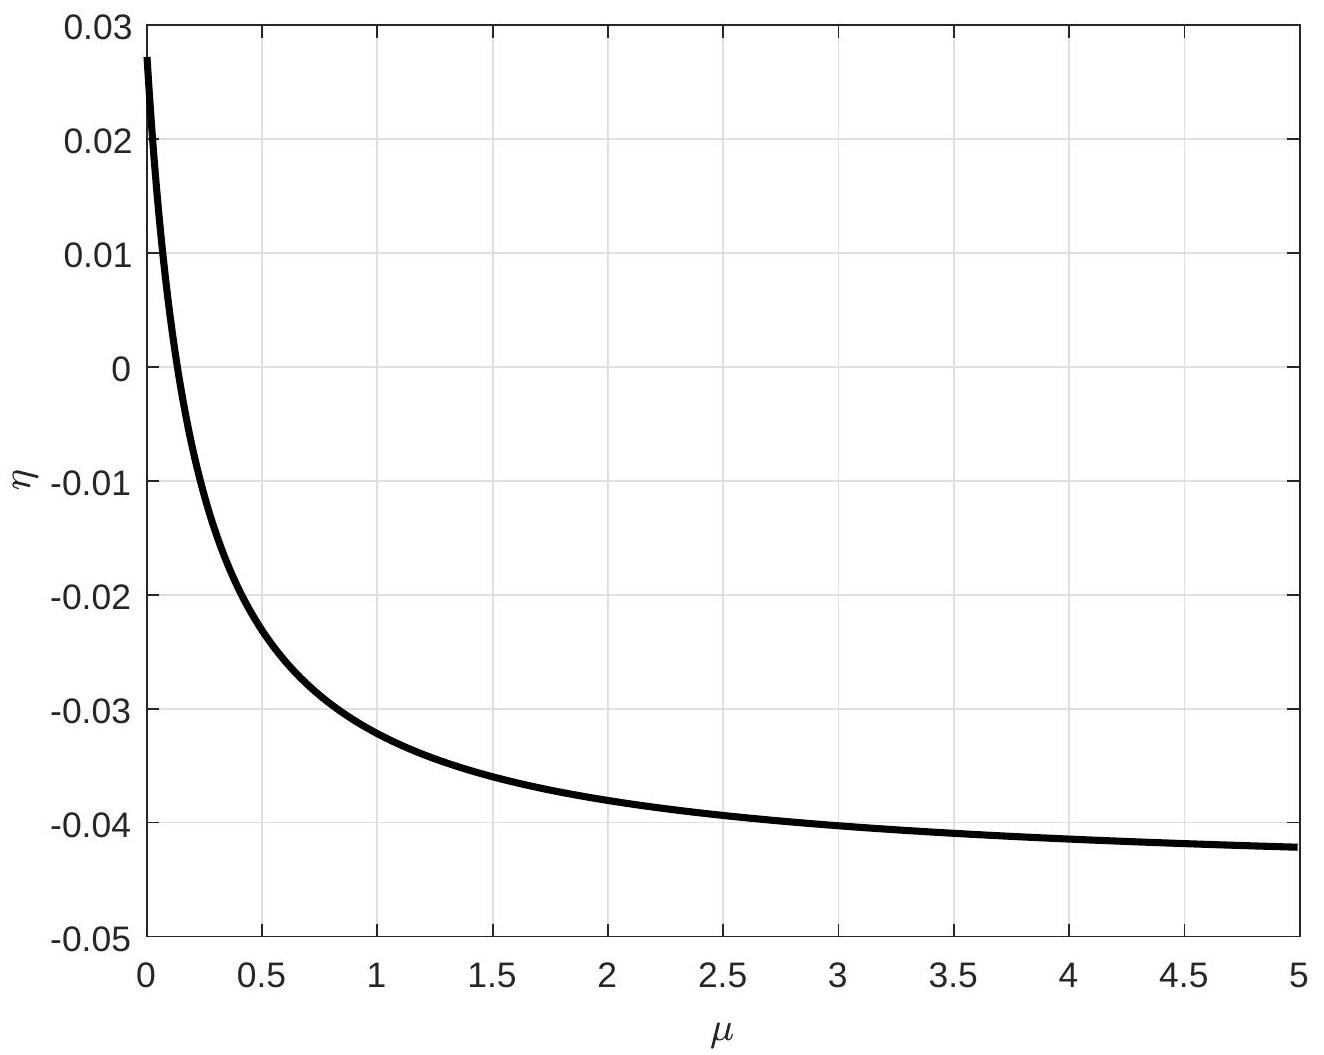
\includegraphics[max width=\textwidth, center]{2024_12_20_23d1456f4ac472ebd83dg-25}

Notes: This figure plots $\eta$ as a function of $\mu$, the welfare weight on the output gap, for the case when $q e_{t}=0$.

\section*{References}
Sims, Eric, Jing Cynthia Wu, and Ji Zhang, "The Four Equation New Keynesian Model," Review of Economics and Statistics, forthcoming.

Woodford, Michael, Interest and Prices: Foundations of a Theory of Monetary Policy, Princeton, NJ: Princeton University Press, 2003.


\end{document}